%% $RCSfile: using.tex,v $
%% $Revision: 1.1 $
%% $Date: 2010/04/23 01:57:05 $
%% $Author: kevin $
%%
% \chapter{Assumptions}
% 
% 
% 
% \section{Static deployment vs. Dynamic deployment}
% As virtual machine technology and infrastructure-as-a-service (IaaS) are becoming
% more and more popular. Dynamic Web service deployment become possible \cite{kemps2012dynamic}. On the other hand, static deploymdent is 
% still the mainstream because of a majority
% of Web service are deployed on local infrastructure \cite{He}. In this paper, we made an
% assumption that WSPs is deployed statically.
% 




\chapter{BPSO for Web Service Location Allocation: An Aggregating Approach}
\label{C:single}

\section{Introduction}
\label{sec:modelintro}

The aim of Web service location allocation is to deploy services with a minimal cost of services to the candidate locations with low overall network latency. 
This problem considers two conflict objectives: minimizing cost and network latency. In an ideal situation, if WSPs deploy services to all candidate
locations, web service users would receive the lowest latency. However, increasing the number of services means increasing cost. Therefore, the allocation must be considered
carefully. In this chapter, we focuses on developing a binary PSO with an aggregating approach.

We first introduce the data that related to the problem and then model the problem with two objectives. In the second part, we apply a BPSO with 
an aggregating approach to solve the problem. In the experiment, we first design 14 problems with increasing variable sizes 
to test the performance of an algorithm. In addition, two small problems with small variable size are specifically designed for BPSO. 
We conduct experiments on BPSO. The results are discussed carefully from the perspective of convergence, evolution process and overall performance.
% Firstly, this model is based on a web service composition assumption, where all atomic services are composed to provide functionalities. Particularly,
% all atomic services are from a single WSP. In his model, an \textbf{\textit{atomic service demand}} denotes the number of request of an atomic Web service
% which is equivalent to \textbf{\textit{service invocation frequency $F$}} mentioned later in this chapter. 
% 
% The model obtain this value according to composition workflows, for example, a WSP has two service composition A and B (Figure \ref{fig:comp}). 
% \begin{figure}[H]
%   \centering
%   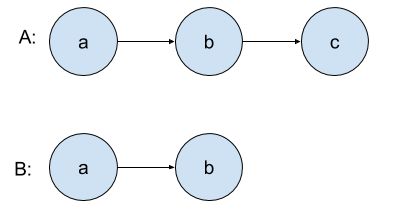
\includegraphics[width=0.7\textwidth]{pics/reasons.png}
%   \caption{Service Composition A and B}
%   \label{fig:comp}
% \end{figure}
% 
% 
% This 
% assumption does not consider atomic services could provide service independently. In other words, this model does not consider standalone Web services.
% Secondly, a major input data \emph{atomic service demand} which indicates the popularity of a service is calculated based on assuming 20\% Web services account for 80\% of overall service requests.
% There is no validation for this assumption. Therefore, two problems may occur when applying this model on a real world problem.
% 
% \begin{enumerate}
%  \item The standalone Web services can not be modeled.
%  \item Only 20\% of Web services are taken into account.
% \end{enumerate}
% 
% It is obvious this model is not general enough to solve real world problems. 
% Hence, this chapter addresses Objective 1, aiming at developing a general model for Web service location-allocation problem.
% The model is not only more generalized but also could be easy to applied in EC algorithms. The model is presented in Section \ref{sec:fitness}. 
% In order to validate the model and provide a baseline of the optimized solution, we developed a single objective BPSO
% to accomplish this task. In BPSO, we use a linear aggregation method to combine two objectives into a $Fitness$. We use the normalized objectives
% to present the results.

\section{Problem Description and Model Formulation}
In the previous study, Huang \cite{EnhancedGenetic} developed a model of Web service location allocation. His approach considers one objective, minimizing network latency. In contrast,
our approach considers the Web service location allocation as a multi-objective problem with two potentially conflicting objectives, minimizing cost and network latency. In this section, we first describe the Web service location allocation problem in detail.  Then we introduce the model formulation.

\subsection{Problem Description}
For service location allocation problem, we need information of service invocation frequency, network latency, and service deployment cost.
Assume a set of $S = \{ s_{1}, s_{2}, \dots,  s_{m}\}$ services are
requested from a set of user centers $I = \{ i_{1}, i_{2}, \dots,  i_{n} \}$. 
WSPs allocate services to a set of candidate locations $J = \{ j_{1}, j_{2}, \dots,  j_{k} \}$.

In this paper, we will use the following matrices.
\begin{center}
{
%\centering
	\footnotesize
	\begin{tabular}{l*{2}{l}r}
		\hline
		\textbf{Matrices} \cr
		$L$ & server network latency matrix $L = \{l_{ij}\}$ \cr
		$A$ & service location matrix $A = \{a_{sj}\}$ \cr
		$F$ & service invocation frequency matrix $F = \{f_{is}\}$ \cr
		$C$ & cost matrix $C = \{c_{sj}\}$ \cr
		$R$ & user response time matrix $R = \{r_{is}\}$ \cr
		\hline
	\end{tabular}
%\\
}
\end{center}

A \emph{service invocation frequency matrix}, $F= [f_{is}]$, is used to record services invocation frequencies from user centers to services. For example, $f_{13}$ = 85 denotes service $s_{3}$ being called 85 times from $i_1$ in a period of time.

% \parbox{.45\linewidth}{
% {\centering
% $
% F = \bbordermatrix{~ & s_{1} & s_{2} & s_{3}  \cr
% 					i_{1}	&120 &35 &56	\cr
% 					i_{2}	&14  &67 &24 \cr
% 					i_{3}	&85 &25 &74 \cr}
% $
% \\}
% }
% \parbox{.45\linewidth}{
% {\centering
% $
% L = \bbordermatrix{~ & j_{1} & j_{2} & j_{3} \cr
% 					i_{1}	&0 &5.776 &6.984	\cr
% 					i_{2}	&5.776  &0 &2.035 \cr
% 					i_{3}	&0.984 &1.135	&2.3 \cr}
% $
% \\}
% }

A \emph{network latency matrix} $L = [l_{ij}]$, is used to record network latencies from user centers to 
candidate locations. For example, the network latency between user center $i_{2}$ with candidate location $j_{1}$ 
is 5.776s. These data could be collected by monitoring network latencies \cite{6076756} \cite{5552800}.

A \emph{cost matrix}, $C = [c_{sj}]$, is used to record the fixed deployment fees at candidate locations, 
where $c_{sj}$ is an integer that indicates the fixed deployment fee at a candidate location. 
For example, $c_{12} = $ 80 denotes the cost of deploying service $s_{1}$ at candidate location $j_{2}$ is 80 cost units.
% 
% \parbox{.45\linewidth}{
% {\centering
% $
% C = \bbordermatrix{~ & j_{1} & j_{2} & j_{3}\cr
% 					s_{1}	&130 &80 &60\cr
% 					s_{2}	&130  &80 &60\cr
% 					s_{3}	&130 &80 &60\cr}
% $
% \\}
% }
% \parbox{.45\linewidth}{
% {\centering
% $
% A = \bbordermatrix{~ & j_{1} & j_{2} & j_{3}\cr
% 					s_{1}	&0 &1 &0	\cr
% 					s_{2}	&0  &0 &1	\cr
% 					s_{3}	&1 &1 &0	\cr}
% $
% \\}
% }

A \emph{service location matrix} $A = [a_{sj}]$ denotes whether the service $s$ is deployed at a candidate location $j$ with 1 denotes deployment, 0 denotes no deployment. 
Service location matrix $A$ is the output matrix. Therefore, it is initially unknown.


A \emph{response time matrix}  $R = [r_{is}]$ denotes the response time from user centers to services. It can be calculated
by using service location allocation matrix $A = [a_{sj}]$ and network latency matrix $L = [l_{ij}]$ according to Equation (\ref{eq:response}).

{\centering
	\begin{equation}
	\label{eq:response}
		r_{is} = \min\{l_{ij} \mid j \in \{1, 2, ..., k\} \text{ and } a_{sj} = 1\}
	\end{equation}
\\}
For example, we can calculate overall network latency by using the two example matrices $L$ and $A$ presented above to construct the response time matrix $R$. 
For each service $s$, by checking matrix $A$, we can find out which location the service has been deployed.
Then we check matrix $L$, to find out its corresponding latency to each user center $i$. If there is
more than one location, then the smallest latency is selected. 

% Therefore, we can construct the response time matrix $R$ as:
% 
% {\centering
% $
% R = \bbordermatrix{~ & s_{1} & s_{2} & s_{3}\cr
% 					i_{1}	&5.776 &6.984 &0	\cr
% 					i_{2}	&0  &2.035 &0	\cr
% 					i_{3}	&1.135 &2.3 &0.984	\cr}
% $
% \\}

\subsection{Model Formulation}
We set service location allocation matrix $A = a_{sj}$ be the decision variable. 
$$
		a_{sj} = 
		\begin{cases}
			1 & \quad \text{service } s \text{ deploy in location } j\\
			0 & \quad \text{otherwise} \\
		\end{cases}
$$

We design two objective functions and one constraint.
\begin{equation}
\begin{aligned}
& {\text{minimize}}
& &  Cost = \sum\limits_{s \in S} \sum\limits_{j \in J} c_{sj} a_{sj},\\
& & & Latency = \sum\limits_{i \in I} \sum\limits_{s \in S} r_{is}  f_{is}\\
& \text{subject to}
& & \displaystyle \sum_{j} a_{sj} \geqslant 1
\end{aligned}
\end{equation}

\emph{Cost} calculates the overall cost of deployed services, where $c_{sj}$ is the cost of deployed service $s$ at candidate location $j$, $a_{sj}$ represents whether service $s$ is allocated to candidate location $j$. The sum of the multiplication of 
D$c_{sj}$ and $a_{sj}$ is the total deployment cost.\end{flushleft}

% \begin{flushleft}For example, we use the above mentioned matrices $C$ and $A$.\end{flushleft}
%   $$
%       \begin{align}
% 	Cost &= c_{11} * a_{11} + c_{12} * a_{12} + c_{13} * a_{13} + ... + c_{33} * a_{33} \\
% 	&= 130 * 0 + 80 * 1 + 60 * 0 + ... + 54 * 0 \\
% 	&= 228 
%       \end{align}
%   $$

\emph{Latency} calculates the overall network latency. Where $r_{is}$ 
denotes the response time from a user center $i$ to a web service $s$ and $f_{is}$ is the invocation frequency of a user center $i$ to a web service
$s$.

% \begin{flushleft}For example, we use the above mentioned matrices $F$ and $R$.\end{flushleft}
%       $$
%       \begin{align}
% 	Latency &= f_{11} * r_{11} + f_{12} * r_{12} + f_{13} * r_{13} + ... + f_{33} * r_{33} \\
% 	&= 120 * 5.776 + 6.984 * 35 + 0 * 56 + ... + 0.984 * 74\\
% 	&= 1300.696
%       \end{align}
%       $$

\begin{flushleft}The constraint requires that each web service is deployed in at least one location.\end{flushleft}

\section{Binary Particle Swarm Optimization}
\subsection{Particle Representation}
\label{sec:rep}

As seen from the above section, Web service location allocation problem can be described with a set of matrices with $F, L, C$ as input, $A$ as output, $min(cost)$ and $min(latency)$ as objectives.
In order to provide a baseline of optimization solutions, we adopt the original BPSO to encode allocation solutions as particles. 
We encode a flatten matrix as the particle representation.
That is, all row vectors in a matrix are concatenated from top row to bottom row to construct a vector.
 Instead of directly using matrix-based representation, it uses a flattened matrix.
 
 \begin{figure}[H]
 \centering
   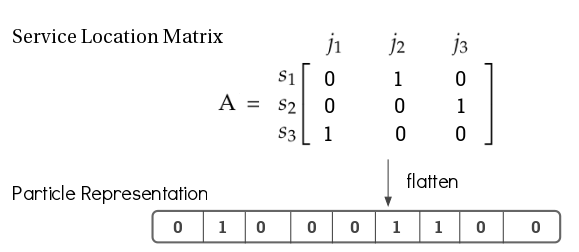
\includegraphics[width=0.7\textwidth]{pics/psorepresentation.png}
   \caption{BPSO particle representation}
   \label{fig:flatten}
 \end{figure}
 
 \subsection{Fitness Function}
To measure the goodness of solutions we need fitness functions.
We employ a linear aggregating method to combine all normalized objectives into one value, with a weight assigned to each
objective to indicate its relative importance (Equation \ref{eq:Fitness}).

Since the maximum and minimum values for total cost and total latency are deterministic, we use exhaustive search to
find out the $Latency_{max}$. $Latency_{min}$ is achieved by deploying all web services to all candidate locations.
$Cost_{min}$ is the cost of allocating each of web services at a location that leads to the minimal cost 
and $Cost_{max}$ is the cost of allocating each web service to all the locations.
 \begin{equation}
 	\label{eq:cost_prime}
 	Cost' = \frac{Cost - Cost_{min}}{Cost_{max} - Cost_{min}}
 \end{equation}
 
 \begin{equation}
 	\label{eq:latency_prime}
 	Latency' = \frac{Latency - Latency_{min}}{Latency_{max} - Latency_{min}}
 \end{equation}

\begin{equation}
\label{eq:Fitness}
	Fitness = w * Latency' + (1 - w) * Cost'
\end{equation}

\subsection{Algorithm}
The key step is updating of $pbest$ and $gbest$. The $pbest$ of a particle is updated when its current fitness is smaller than previous $pbest$.  
The $gbest$ is the best solution in all $pbest$. Hence, it is updated when a current $pbest$ is smaller than previous $gbest$. 

\begin{minipage}{1.0\linewidth}
 \begin{algorithm}[H]
 \footnotesize
	\caption{BPSO for Web Service Location Allocation}
	\textbf{Inputs:} \\
		Cost Matrix $C$, \\
		Server network latency matrix $L$, \\
		Service invocation frequency matrix $F$ \\

	\textbf{Outputs:}
		Pareto Front

	\begin{algorithmic}[1]
	\State Initialize the position and velocity of particles in the swarm ($Swarm$).
	\Repeat
	  \State Evaluate $Swarm$ with fitness functions, each particle has two objectives $Cost$ and $Latency$;
	  \State Use linear normalization to normalize each particle's objectives
	  \State Calculate a combined fitness value $F = (1 - w) Cost' + w * Latency' $;
	  \State Update $pbest$ and $gbest$;
	  \State Update velocity and position;
	\Until{ maximum iterations is reached}
	\State Return $Swarm$
	\end{algorithmic}
	\label{alg:BPSO}
\end{algorithm}
\end{minipage}



 
\subsection{Constraint Handling}
We model the Web service location allocation problem with one constraint, it requires each web service to be deployed to at least one location.
Because of the constraint, not all web service location allocation matrices are valid. Therefore, we need a constraint handling method to restrict the population generated by the algorithm.
\label{sec:constraint}
There are five categories of constraint handling summarized by Coello \cite{coello2002theoretical}, 
\begin{enumerate}
	\item Penalty functions
	\item Special representation and operators
	\item Repair algorithms
	\item Separation of objectives and constraints
	\item Hybrid Methods
\end{enumerate}
 
BPSO applies a ``death penalty'' in constraint handling which is a special case of penalty function \cite{coello2002theoretical}.
The invalid solutions are assigned the maximum fitness value. That means the penalized 
particle will lose chance to be the global best in the current generation. This penalty function prevents the swarm from moving to invalid regions.

\begin{equation}
\label{eq:death}
		Fitness(x_{id}) = 
		\begin{cases}
			1 & \quad \text{if violate constraint} \\
			\text{normalized fitness value} & \quad \text{otherwise} \\
		\end{cases}
\end{equation}


The invalid particles are remaining in the 
population. In the next generation, they could move out of invalid regions and
become valid again.

% ``Death penalty'' method in PSO is not considered as harmful as in GA 
% since all the invalid particles are still remained in the population.


% We consider two basic constraints. The first is service number constraint, it requires that each service is deployed in at least one location.



% The second constraint is the cost constraint which predefined the upper boundary of the total cost.
% An integer number $CostLimitation$ is defined.
% 
% 
% \begin{equation}
% 	\sum\limits_{s \in S} \sum\limits_{j \in J} C_{sj}  A_{sj} \leq CostLimitation
% \end{equation}


\section{Experiments and Results}
\subsection{Datasets}
\label{sec:datasets}
This project is based on both real world datasets and stimulated datasets. 
In this project, there are mainly three attributes that needs to be provided, 
network latencies between candidate locations and user centers,  server rental cost in candidate locations 
and web service invocation frequencies information.

Table \ref{tab:problem} shows fourteen problems, 
which are either generated from existing data or generated from a normal distribution (introduced in Section \emph{Cost}, \emph{Service Invocation Frequency} and \emph{Network Latency}).  
The problems are in increasing size and difficulty which are used as representative samples of the Web service 
location allocation problem.

\begin{table}[H]
\footnotesize
\centering
\caption{Problem set}
\label{tab:problem}
\begin{tabular}{l|c|c|c}
\hline
Datasets   & \multicolumn{1}{l|}{\begin{tabular}[c]{@{}l@{}}No. of \\ Services\end{tabular}} & \multicolumn{1}{l|}{\begin{tabular}[c]{@{}l@{}}No. of \\ Candidate Locations\end{tabular}} & \multicolumn{1}{l}{\begin{tabular}[c]{@{}l@{}}No. of \\ user centers\end{tabular}} \\ \hline
Problem 1  & 20                                                                             & 5                                                                                         & 10                                                                                  \\ \hline
Problem 2  & 20                                                                             & 10                                                                                        & 10                                                                                  \\ \hline
Problem 3  & 50                                                                             & 15                                                                                        & 20                                                                                  \\ \hline
Problem 4  & 50                                                                             & 15                                                                                        & 40                                                                                  \\ \hline
Problem 5  & 50                                                                             & 25                                                                                        & 20                                                                                  \\ \hline
Problem 6  & 50                                                                             & 25                                                                                        & 40                                                                                  \\ \hline
Problem 7  & 100                                                                            & 15                                                                                        & 20                                                                                  \\ \hline
Problem 8  & 100                                                                            & 15                                                                                        & 40                                                                                  \\ \hline
Problem 9  & 100                                                                            & 25                                                                                        & 20                                                                                  \\ \hline
Problem 10 & 100                                                                            & 25                                                                                        & 40                                                                                  \\ \hline
Problem 11 & 200                                                                            & 25                                                                                        & 40                                                                                  \\ \hline
Problem 12 & 200                                                                            & 25                                                                                        & 80                                                                                  \\ \hline
Problem 13 & 200                                                                            & 40                                                                                        & 40                                                                                  \\ \hline
Problem 14 & 200                                                                            & 40                                                                                        & 80                                                                                  \\ \hline
\end{tabular}
\end{table}


\subsubsection{Cost}
\label{sec:costdata}
A WSP rents servers from Web Server Hosting Providers (WSHPs). 
The rental fee  normally includes fixed deployment fees and variable fees based on usage \cite{Sun:2003:}. 
Fixed deployment fees  refer to the monthly payment for a specific server plan from a WSHP. 
Fixed deployment fees  mainly depend on the quantity, namely the number of servers and quality features include computing power, 
reliability, network bandwidth. Variable fees include extra charges from exceeded storage and other limits.
This project would only consider fixed deployment fees. The cost is under the following assumptions, 
the fixed deployment of web services in the same candidate location are the same. 
This project uses stimulated cost by randomly generating from a normal distribution where mean is 100, standard deviation is 20. 

\subsubsection{Service Invocation Frequency}
\label{sec:frequencydata}
Frequency refers to the invocation frequency from a location to a web service within a certain period of time \cite{Huang:2013:}. 
This project uses simulated frequency data that randomly generate from an uniform distribution from 1 to 120.

\subsubsection{Network Latency}
\label{sec:latencydata}
Network latency denotes the latency between a user center and a candidate location. 
The network latency depends on not only the geographic locations but also the topological locations. 
The project sees the network topology as a black box and uses network latency as the network quality measurement. 
A network latency data set is provided by WS-DREAM \cite{6076756} \cite{5552800}, 
it measures the network latency between 339 user centers to 5825 candidate locations. 
The provided data is represented as a matrix.

$$
Latency Data = \bbordermatrix{~ & j_{1} & j_{2} & \dots &j_{5825}  \cr
					i_{1}	&0.52 &3.8 &\dots &5.6	\cr
					i_{2}	&1.4  &6.7 &\dots &2.4 \cr
					\vdots  &\vdots &\vdots &\ddots &\vdots \cr
					i_{339}	&8.5 &2.5 &\dots &7.4 \cr}
$$


The project uses subsets of the matrix. 
It randomly selects a subset of the matrix as the latency matrix $L$, 
where the number of user centers and candidate locations are defined by experimental design. 
The only selection constraint is the network latency value which can not be $Null$ value since we assume a WSP provides complete information.

For example, the experiment requires an $N * M$ latency matrix, that is, $N$ user centers and $M$ candidate locations.
In the first step, it randomly selects an $N * M$ matrix from the data matrix. In the second step, it replaces the row which has $Null$ value with a random row. 
Repeat the second step until all matrix has no $Null$ value.
% 
% Optimization is a process that highly depends on input data. 
% Therefore, it is important to understand the distribution of the network latency data.
% As figure \ref{fig:density} shows, 
% 
% \begin{figure}[H]
%   \centering
%   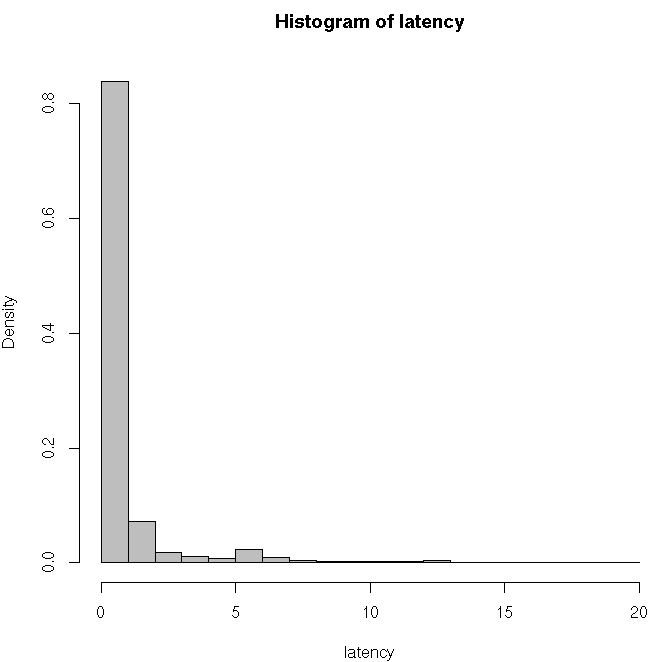
\includegraphics[width=0.5\textwidth]{pics/latency_density.png}
%   \caption{latency density}
%   \label{fig:density}
% \end{figure}
% 
% \begin{table}[H]
% \footnotesize
% \centering
% \caption{Statistics of Latency data}
% \label{tab:details}
% \begin{tabular}{|l|l|l|l|l|l|}
% \hline
% Min   & 1st Quartile & Median & Mean   & 3rd Quartile & Max  \\ \hline
% 0.001 & 0.156        & 0.32   & 0.9086 & 0.6720       & 20.0 \\ \hline
% \end{tabular}
% \end{table}
% 
% The range of network latency is  [0, 20].
% Over 90\% of the latency data are concentrated on [0, 2]. 

\subsubsection{Small Problems}
Two small problems are designed to validate that our proposed BPSO algorithm for web service allocation is capable of finding near optima solutions.
The two small problems are using small datasets so that it is feasible to use
a brute-force algorithm (e.g. evaluate all permutation of the solutions) to find the optimal solutions.

We define the small problems as follows:

\begin{table}[!htb]
\centering
\caption{Small Problems}
\label{my-label}
\begin{tabular}{|l|c|c|c|}
\hline
Datasets        & \multicolumn{1}{l|}{\begin{tabular}[c]{@{}l@{}}No. of \\ Services\end{tabular}} & \multicolumn{1}{l|}{\begin{tabular}[c]{@{}l@{}}No. of \\ Candidate Locations\end{tabular}} & \multicolumn{1}{l|}{\begin{tabular}[c]{@{}l@{}}No. of\\ User centers\end{tabular}} \\ \hline
Small problem 1 & 2                                                                               & 3                                                                                          & 2                                                                                  \\ \hline
Small problem 2 & 4                                                                               & 4                                                                                          & 3                                                                                  \\ \hline
\end{tabular}
\end{table}

The search space of these two small problems can be calculated as follows, 
because of each entry in the service location allocation matrix could be 0 or 1. 
The search space for problem 1 is $2^6 = 64$, problem 2 is $2^{16} = 65536$.

Small problem 1:

\parbox{.3\linewidth}{
{\centering
$
F = \bbordermatrix{~ & s_{1} & s_{2}  \cr
					i_{1}	&10 &116	\cr
					i_{2}	&119 &95 \cr}

$
\\}
}
\parbox{.3\linewidth}{
{\centering
$
L = \bbordermatrix{~ & j_{1} & j_{2} & j_{3} \cr
					i_{1}	&0 &0.3 &0.5	\cr
					i_{2}	&0.4  &0 &0.6 \cr}
$
\\}
}
\parbox{.3\linewidth}{
{\centering
$
C = \bbordermatrix{~ & j_{1} & j_{2} & j_{3}\cr
					s_{1}	&98 &72 &144\cr
					s_{2}	&98  &72 &144\cr}
$
\\}
}

Small problem 2:

\parbox{.5\linewidth}{

$
F = \bbordermatrix{~ & s_{1} & s_{2} & s_{3} \cr
					i_{1}	&58 &2 &34 &93	\cr
					i_{2}	&104 &111 &56 &70 \cr
					i_{3}	&87 &25 &42 &9 \cr}
$


}
\parbox{.5\linewidth}{

$
L = \bbordermatrix{~ & j_{1} & j_{2} & j_{3} & j_{4}\cr
					i_{1}	&0 &0.125 &0.044 &0.054	\cr
					i_{2}	&0.125  &0 &3.7 &0.13 \cr
					i_{3}	&0.044  &3.7 &0 &0.36 \cr}
$

}

$
C = \bbordermatrix{~ & j_{1} & j_{2} & j_{3} & j_{4}\cr
					s_{1}	&70  &69 &91 &120\cr
					s_{2}	&70  &69 &91 &120\cr
					s_{2}	&70  &69 &91 &120\cr
					s_{2}	&70  &69 &91 &120\cr}
$


\subsection{Experiment Design}
We conduct experiment on Problems 1 $\sim$ 6 and two small problems.

The parameters of the BPSO algorithms are set as follows: $c_1$ = 2, $c_2$ = 2, population size is 50 and the max number of iteration is 50. 
We assume both objectives are equally important, therefore, a weight $w$ for linear aggregation is set to 0.5. 


\subsection{Results}
We first present the convergence curves of BPSO in Figure \ref{fig:convergence}. In each generation, we calculate the average of the best solutions of 40 runs .
The $x$ axis denotes the 
generation and $y$ axis denotes the fitness value. As it is shown, the initial fitness value is large because 
the particles are randomly initialized.  Along with the evolution, the fitness values follow a decreasing trend. It means that the BPSO finds better solutions in each generation.


\begin{figure}[!h]
   \centering
   \begin{subfigure}{0.3\textwidth}
       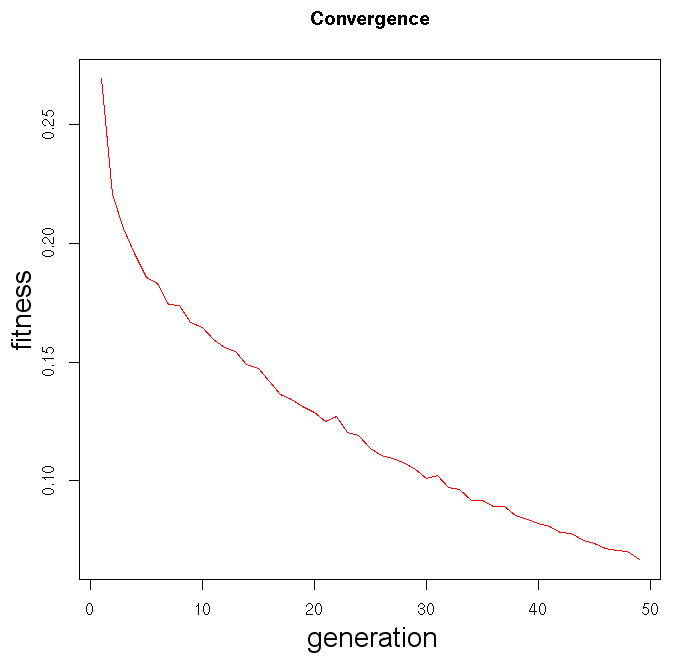
\includegraphics[width=\textwidth]{pics/convergence1.png}
	   \caption{Problem 1}
   \end{subfigure}
   \begin{subfigure}{0.3\textwidth}
       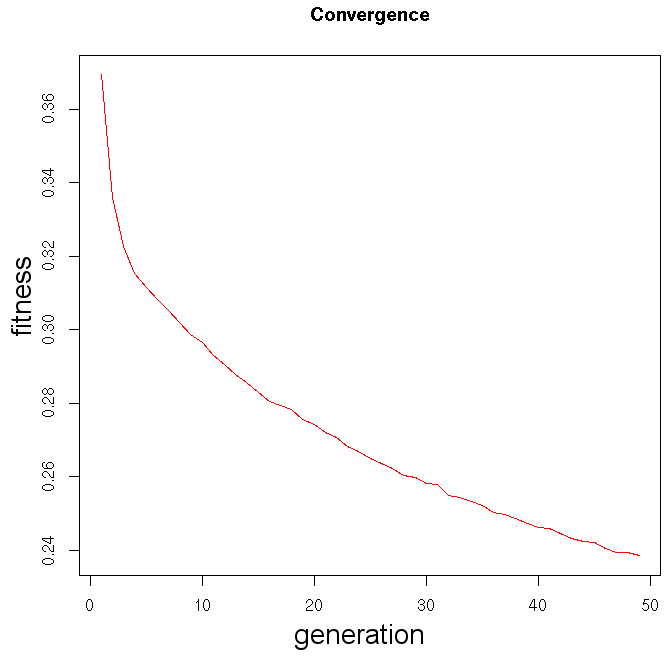
\includegraphics[width=\textwidth]{pics/convergence2.png}
	   \caption{Problem 2}
   \end{subfigure}
   \begin{subfigure}{0.3\textwidth}
       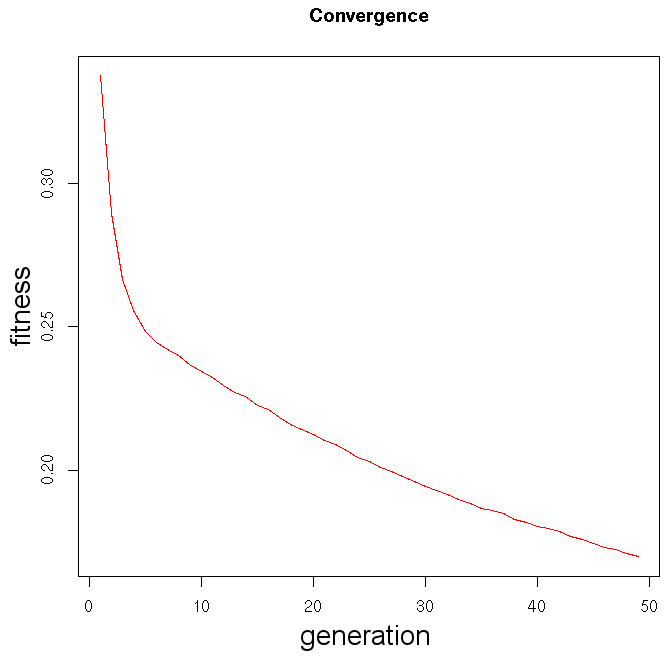
\includegraphics[width=\textwidth]{pics/convergence3.png}
	   \caption{Problem 3}
   \end{subfigure}
   \begin{subfigure}{0.3\textwidth}
       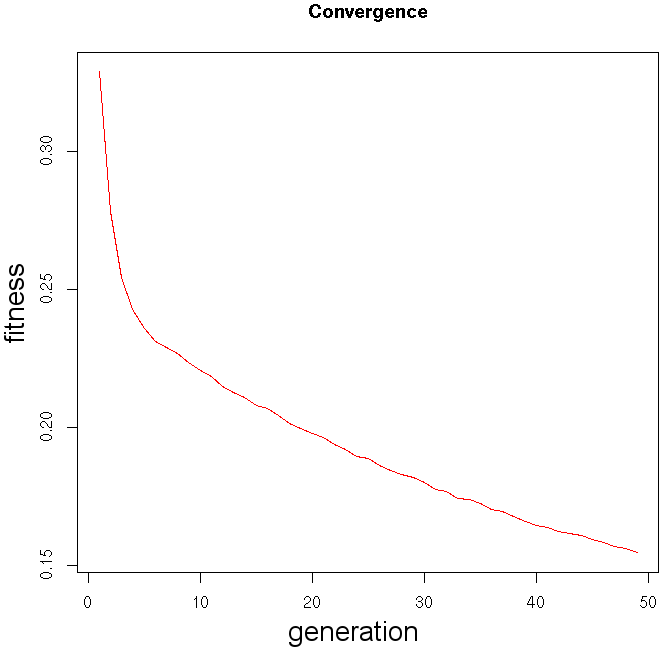
\includegraphics[width=\textwidth]{pics/convergence4.png}
	   \caption{Problem 4}
   \end{subfigure}
      \begin{subfigure}{0.3\textwidth}
       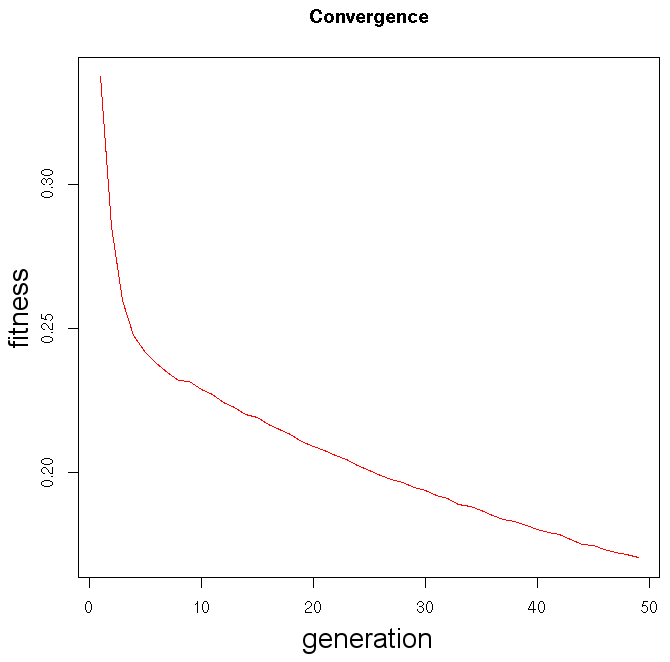
\includegraphics[width=\textwidth]{pics/convergence5.png}
	   \caption{Problem 5}
   \end{subfigure}
      \begin{subfigure}{0.3\textwidth}
       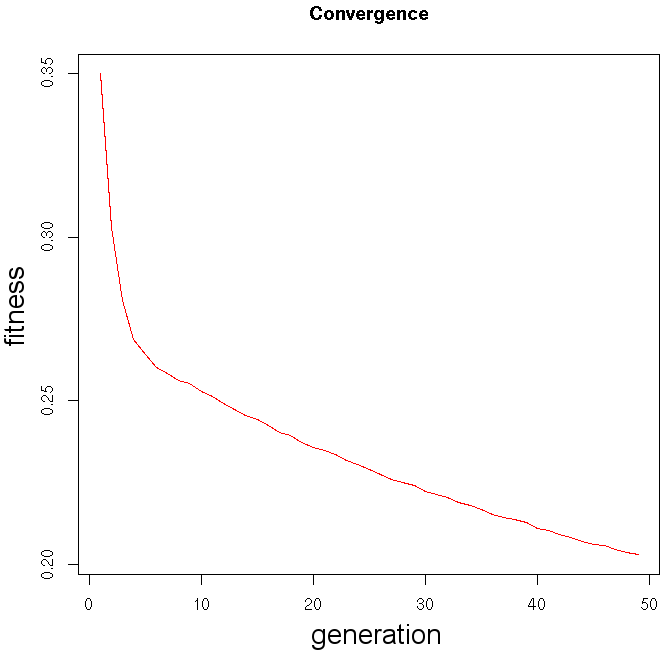
\includegraphics[width=\textwidth]{pics/convergence6.png}
	   \caption{Problem 6}
   \end{subfigure}
   \caption{Convergence curve by averaging 40 independent runs}
   \label{fig:convergence}
\end{figure}


We could also see the  evolutionary process by observing Figure \ref{fig:bpso_evolve} where it shows
the solutions from 10th, 20th, 30th, 40th and 50th generation of problem 1 $\sim$ 4. It shows a 
pattern that the solutions are moving to a low fitness region. We could observe this pattern clearly from problem 1 and 2. As solutions move from blue region to black region. It is not so obvious in problem 3 
and 4. The reason is that the BPSO could not find better solutions so the swarm schooling along the borderline which every solutions are equally good.
\begin{figure}[!h]
   \centering
   \begin{subfigure}{0.4\textwidth}
       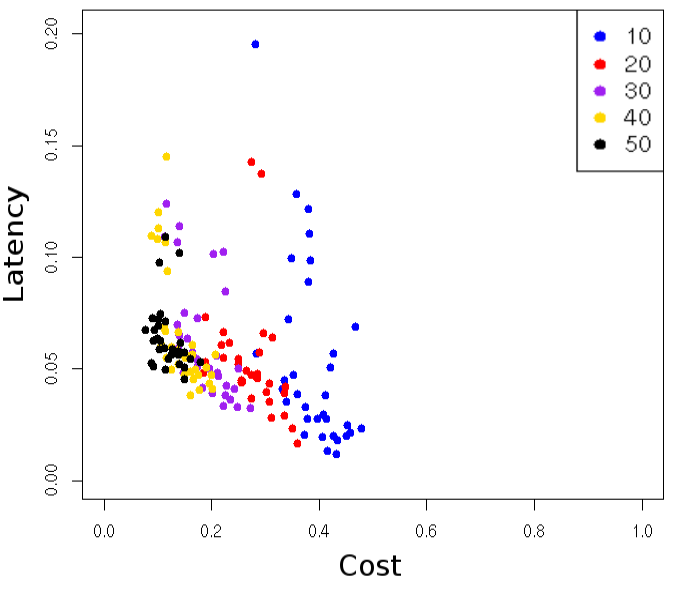
\includegraphics[width=\textwidth]{pics/binaryevolve1.png}
	   \caption{Problem 1}
   \end{subfigure}
   \begin{subfigure}{0.4\textwidth}
       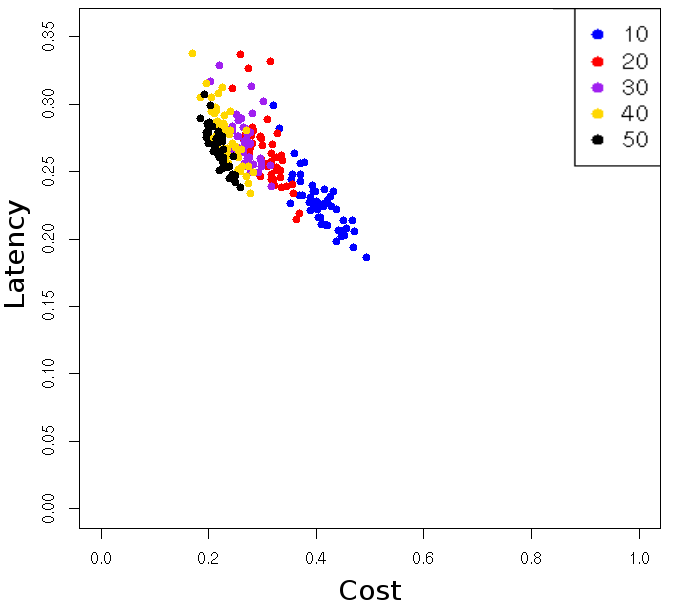
\includegraphics[width=\textwidth]{pics/binaryevolve2.png}
	   \caption{Problem 2}
   \end{subfigure}
   \begin{subfigure}{0.4\textwidth}
       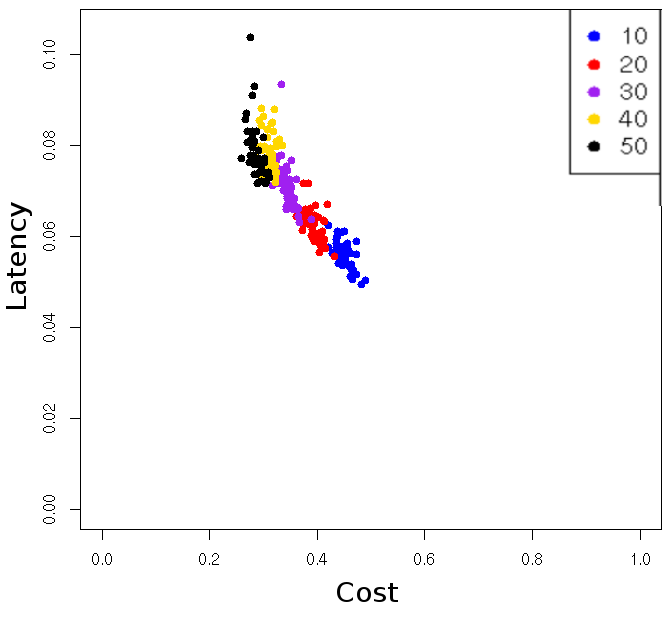
\includegraphics[width=\textwidth]{pics/binaryevolve3.png}
	   \caption{Problem 3}
   \end{subfigure}
   \begin{subfigure}{0.4\textwidth}
       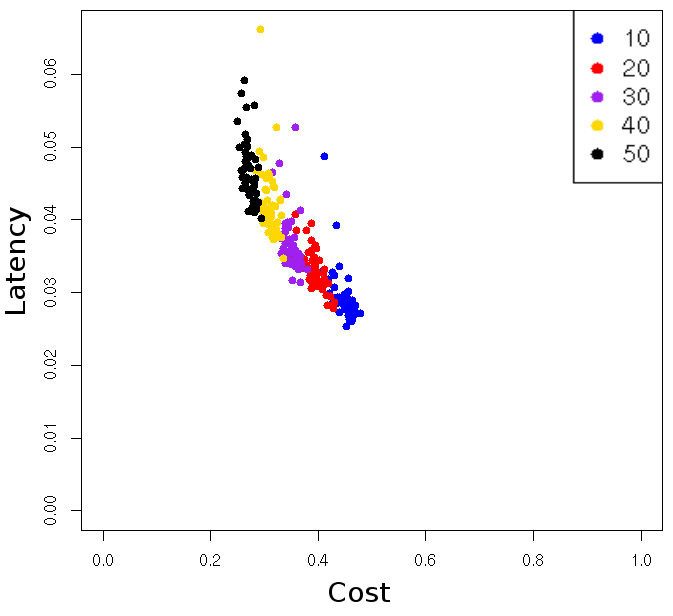
\includegraphics[width=\textwidth]{pics/binaryevolve4.png}
	   \caption{Problem 4}
   \end{subfigure}

   \caption{BPSO Optimization Process}
   \label{fig:bpso_evolve}
\end{figure}



In BPSO, each particle is a solution. We plot the particles from the last
generation with two objectives in Figure \ref{fig:bpso_experiments} . The red points denote the solutions and the marked point denotes the solution with best fitness value. We draw a blue line with $slope = 1 $ passing through it.

We found that, as we set the $weight$ in aggregating method to 0.5, the solutions are evolved
along the direction of $y = x$. 
The solutions scattered along with the plane that orthogonal to the evolve direction. As there are two objectives in the problem, the plane is a line with $slope = -1$. Problems 2 $\sim$ 6 clearly shows this phenomenon. As we could observe that although the marked point has the best
fitness value, it does not necessarily better than other solutions in the perspective of each objective.
In other words, there are a few non-dominated solutions.
In problem 3 $\sim$ 6, it is clearly that many solutions have lower latency and higher cost than the best fitness solution. 

\begin{figure}[!h]
   \centering
   \begin{subfigure}{0.3\textwidth}
       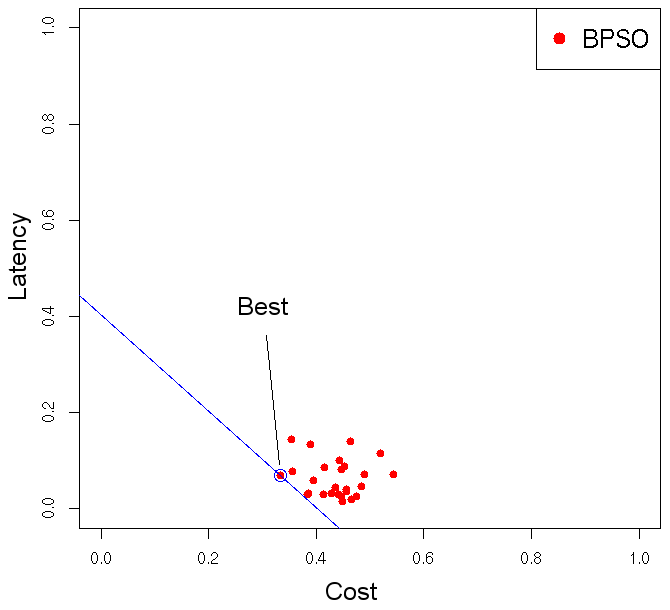
\includegraphics[width=\textwidth]{pics/binary1.png}
	   \caption{Problem 1}
   \end{subfigure}
   \begin{subfigure}{0.3\textwidth}
       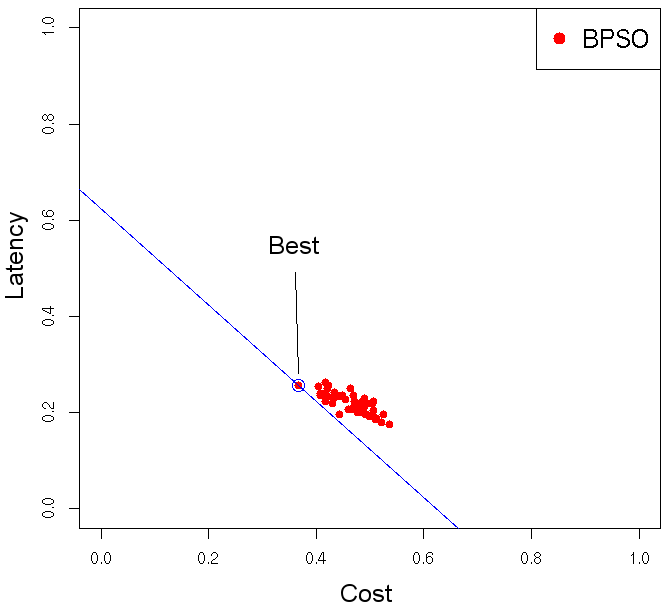
\includegraphics[width=\textwidth]{pics/binary2.png}
	   \caption{Problem 2}
   \end{subfigure}
   \begin{subfigure}{0.3\textwidth}
       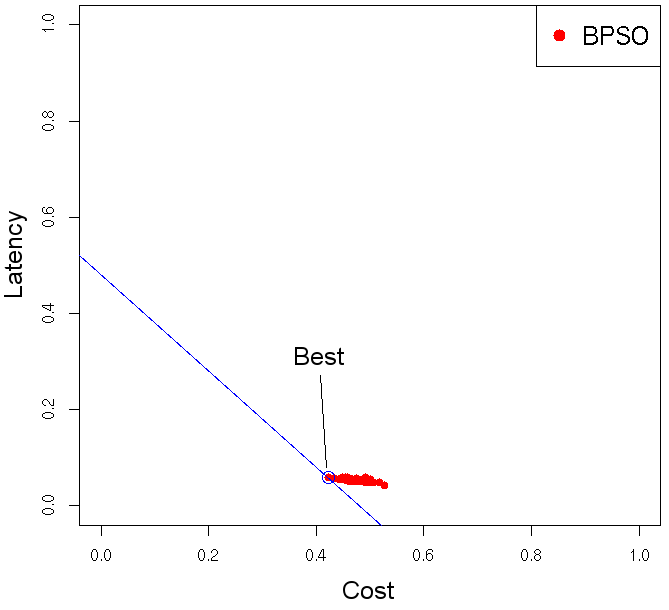
\includegraphics[width=\textwidth]{pics/binary3.png}
	   \caption{Problem 3}
   \end{subfigure}
   \begin{subfigure}{0.3\textwidth}
       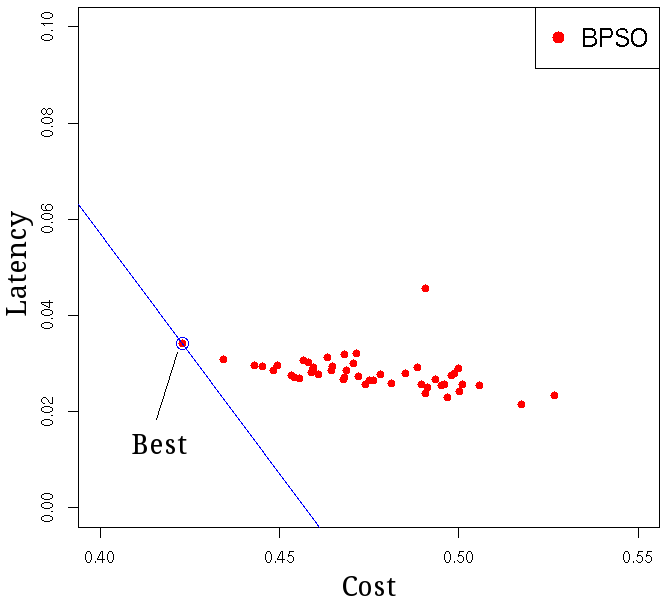
\includegraphics[width=\textwidth]{pics/binary4.png}
	   \caption{Problem 4}
   \end{subfigure}
      \begin{subfigure}{0.3\textwidth}
       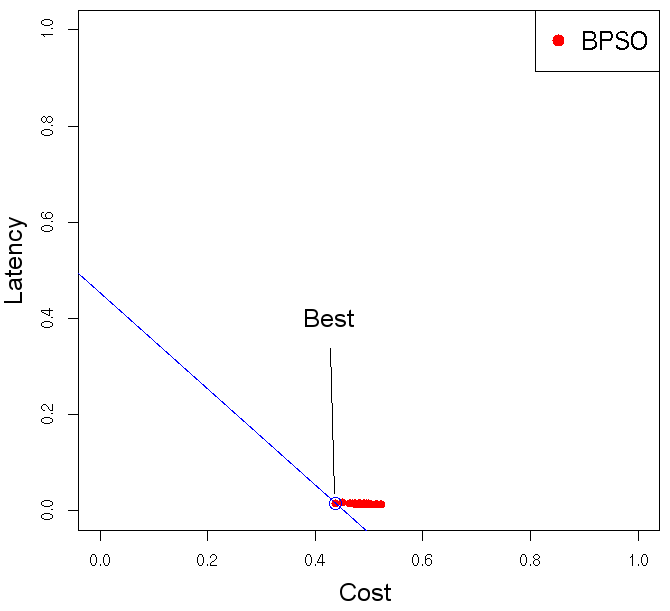
\includegraphics[width=\textwidth]{pics/binary5.png}
	   \caption{Problem 5}
   \end{subfigure}
      \begin{subfigure}{0.3\textwidth}
       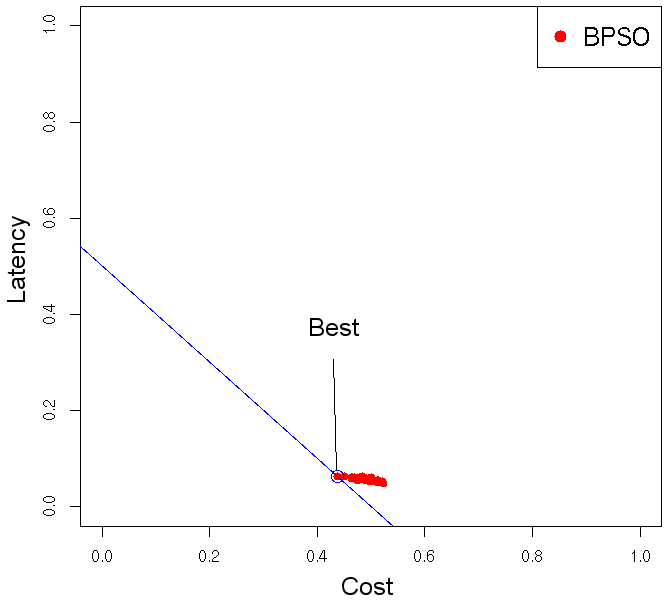
\includegraphics[width=\textwidth]{pics/binary6.png}
	   \caption{Problem 6}
   \end{subfigure}
   \caption{BPSO Experiments: Solutions of Problems 1 $\sim$ 6}
   \label{fig:bpso_experiments}
\end{figure}


For the small problems, the results are presented in Table \ref{tab:small}. We observed, for small problem 1, BPSO converged at a solution 001100, 
for small problem 2, it converged at 1111000000000000.
We convert them to a matrix representation, shown  as $A_1$ and $A_2$,

\begin{table}[!h]
\footnotesize
\centering
\caption{Small problems}
\begin{subtable}{.4\linewidth}
\centering
\caption{Small problem 1}
\begin{tabular}{|l|l|l|}
\hline
     & fitness & particle \\ \hline
1    & 0.099   & 001100   \\ \hline
2    & 0.099   & 001100   \\ \hline
3    & 0.099   & 001100   \\ \hline
4    & 0.099   & 001100   \\ \hline
5    & 0.099   & 001100   \\ \hline
6    & 0.19    & 001101   \\ \hline
7 \sim 50 & 0.099   & 001100   \\ \hline

\end{tabular}

\end{subtable}
\begin{subtable}{.4\linewidth}
\centering
\caption{Small problem 2}

\begin{tabular}{|l|l|l|}
\hline
     & fitness & particle \\ \hline
1    & 0.021   & 1111000000000000   \\ \hline
2    & 0.021   & 1111000000000000   \\ \hline
3    & 0.021   & 1111000000000000   \\ \hline
4    & 0.021   & 1111000000000000   \\ \hline
5    & 0.046   & 1111000001000000   \\ \hline
6    & 0.0735  & 1111000010000000   \\ \hline
7 \sim 50    & 0.021   & 1111000000000000   \\ \hline
\end{tabular}
\end{subtable}
\label{tab:small}
\end{table}


\parbox{.5\linewidth}{

$$
A_1 = \bbordermatrix{~ & j_{1} & j_{2} & j_{3}\cr
					s_{1}	&0 &1 &0	\cr
					s_{2}	&0  &1 &0	\cr}
$$
}
\parbox{.5\linewidth}{

$$
A_2 = \bbordermatrix{~ & j_{1} & j_{2} & j_{3} & j_{4}\cr
					s_{1}	&1 &0 &0 &0	\cr
					s_{2}	&1  &0 &0 &0	\cr
					s_{3}	&1 &0 &0 &0	\cr
					s_{4}	&1 &0 &0 &0	\cr}
$$
}
For each small problem, we applied brute-force algorithm to search for the optimal solution.  
The results have proved PSO found the optimal solutions in both cases.
Therefore, we know BPSO are able to find out optimal solution. For the large datasets, BPSO is able to converge towards the optimal solutions. Unfortunately,
BPSO does not necessarily find optima in every problem because of many reasons,
\begin{enumerate}
	\item Search space is too large.
	\item Not run enough generation to converge.
	\item The algorithm stuck at local optima.
\end{enumerate}

In particular, we notice that in two small problems, all web services are deployed in the same locations. These are special cases which are not frequently
happened. In a practical situation, optimal candidate locations for web services are not necessary the same. 
The choices are highly dependent on the given attributes (latency, invocation frequency and cost).


\section{Discussions}
% In the Section \ref{sec:modelintro}, we discussed the new model overcome two problems faced by Huang's model.
% \begin{enumerate}
%  \item The standalone Web services can not be modelled.
%  \item Only 20\% of Web services are taken into account.
% \end{enumerate}
% 
% We resolve these problems by introducing a new input data: invocation frequency.
% Inocation frequency is similar to web page hits and referrals. It simplified the problem by making no assumption of web services' consumer.
% All consumers (human or other services) could contribute to a Web service's invocation frequency.
% This model also make no assumption of the distribution of requests. The invocation frequency naturaly reflect the popularity of a Web service. 

WSPs may have their specific requirements, for example, financial service providers are willing to make more invention to improve the QoS while social network 
service providers prefer less expenditure even it means the decline of QoS. 
As we observed in Figure \ref{fig:bpso_experiments},
clearly, the solutions are lack of diversity. 
This is the major drawback of using an aggregating method to solve multi-objective problems. The linear
aggregating method tries to optimize the overall fitness and ignore each objective. As a consequence, the 
solutions are concentrated on a narrow region.


\section{Summary} 
This chapter first introduces a model for Web service location allocation problem with two objectives.
Second, it presents a BPSO approach which employs an linear aggregating method to combine two objectives. 
The BPSO uses a ``death penalty'' approach. Third, the chapter presents eight experiments over the BPSO  including six normal size problems and two small problems. 
The results shown that BPSO can solve the problem we modeled and provides good 
solutions. However, the drawback of BPSO is that it couldn't provide a variety of choices to let service providers to choose according to their preferences. 
In the next step, we are going to apply a multi-objective PSO approach to treat each objective separately.


\chapter{A Pareto-Front Multi-Objective to Web Service Location Allocation}
\label{C:multi}
\section{Introduction}
In the previous chapter, we modeled the Web service location allocation problem and developed a BPSO with a linear aggregating approach.
The results show BPSO provides good solutions but with insufficient diversity. In order to improve diversity, 
in this chapter, we develop a NSPSO-based approach with two separate fitness functions. 
In addition, in order to show the effectiveness of NSPSO, we also employ a common multi-objective evolutionary algorithm - NSGA-II.
These algorithms are not new, but it is the first time to apply them to the Web service location allocation problem.

The goal of this chapter is to develop a NSPSO-based approach that provides solutions with 
a better diversity.

\section{NSPSO for Web Service Location Allocation}
We applied the NSPSO developed by Li \cite{NSPSO}. The algorithm is shown in Algorithm \ref{alg:NSPSO}. 
The particle representation is a flatten binary matrix which is the same as BPSO (Section \ref{sec:rep}) .
The constraint handling method is also ``death penalty'' as in BPSO (Section \ref{sec:constraint}).


\begin{algorithm}[!h]
	\caption{NSPSO for Web Service Location Allocation}
	\footnotesize
	\textbf{Inputs:} \\
		Cost Matrix $C$, \\
		Server network latency matrix $L$, \\
		Service invocation frequency matrix $F$ \\

	\textbf{Outputs:}
		Pareto Front

	\begin{algorithmic}[1]
		\State Initialize the position and velocity of particles in the swarm ($Swarm$).
		\Repeat
			\State Evaluate each particle with fitness functions;
			\State Identify the particles ($nonDomS$) that have non-dominated solutions in $Swarm$;
			\State Calculate crowding distance of each particle in $nonDomS$;
			\State Sort particles in $nonDomS$ based on the crowding distance;
			\State Copy all the particles in $Swarm$ to a union set ($Union$)
			\For { i = 1 to Population Size (P) }
			  \State update the $pbest$ of particle $i$
			  \State randomly selecting a $gbest$ for particle $i$ from the least crowded solutions in $nonDomS$;
			  \State update the velocity and position of particle $i$;
			  \State add the updated particle $i$ to $Union$ set;
			\EndFor
		\State Identify different levels of non-dominated fronts $F = (F_1, F_2, F_3, \dots)$ in $Union$;
		\State Empty the current $Swarm$ for the next iteration;
		\State $i = 1;$
		\While { $\mid Swarm \mid < P$ }
		  \If { $\mid Swarm \mid + \mid F_i \mid \leq P$}
		    \State add $F_i$ to $Swarm$;
		    \State $i = i + 1$;
		  \EndIf
		  \If {$\mid Swarm \mid + \mid F_i\mid  > P$}
		    \State calculate crowding distance in $F_i$;
		    \State sort particle in $F_i$;
		    \State add the ($P - \mid Swarm \mid$) least crowded particles to $Swarm$;
		  \EndIf
		\EndWhile
		\Until{ maximum iterations is reached}
		\State return the positions of particles in $F_1$;
	\end{algorithmic}
	\label{alg:NSPSO}
\end{algorithm}



\subsection{Fitness Functions}
\label{sec:nspsofitness}
In the previous section, we defined two objective functions \emph{Cost} and \emph{Latency}. Instead of 
combining two objective functions as one fitness function, 
In NSPSO, we would address them as two fitness functions.

 \begin{equation}
 	\label{eq:cost_prime}
 	CostFitness = \frac{Cost - Cost_{min}}{Cost_{max} - Cost_{min}}
 \end{equation}
 
 \begin{equation}
 	\label{eq:latency_prime}
 	LatencyFitness = \frac{Latency - Latency_{min}}{Latency_{max} - Latency_{min}}
 \end{equation}



\section{NSGA-II for Service Location Allocation}
NSGA-II is one of the most popular evolutionary multi-objective technique.
In this section, we investigate a NSGA-II based multi-objective approach for Web service location allocation.
There are two versions of NSGA-II, continuous and discrete. Because the Web service location allocation problem is a binary problem, we adopt the 
discrete version.
Similar to NSPSO, NSGA-II also adopted the two objective functions as the fitness functions.


\subsection{Chromosome Representation}
A chromosome can be used to represent a service location allocation matrix without making any changes.

$$
A = \bbordermatrix{~ & j_{1} & j_{2} & j_{3}\cr
					s_{1}	&0 &1 &0	\cr
					s_{2}	&0  &0 &1	\cr
					s_{3}	&1 &1 &0	\cr}
$$



\begin{algorithm}[!htb]
	\caption{NSGA-II for Web Service Location Allocation}
	\footnotesize
	\label{alg:NSGA2}
	\textbf{Inputs:} \\
		Cost Matrix $C$, \\ 
		Server network latency matrix $L$, \\
		Service invocation frequency matrix $F$ \\

	\textbf{Outputs:}
		Pareto Front:a  set of service allocation matrix $A$

	\begin{algorithmic}[1]
		\State Initialize a $population$ size of $M$;
		\State Evaluate $population$ with fitness functions;
		\State Apply Fast Non-dominated sort and assign a ranking to each chromosome in $population$;
		\State Apply Tournament Selection $childdren$;
		\State Apply crossover and mutation  over $children$;
		\State Apply Repair algorithm;
		\State Combine $population$ and $children$ to $selected$;
		\While{predefined generation}
		    \State Apply fast non-dominated sort on $selected$;
		    \State Generate sets of non-dominated fronts $F = (F_1, F_2, \dots)$;
		    \State Loop (inside) by adding solutions to next generation;
		    \State starting from the $F_1$ until the $M$ individuals found;
		    \State Evaluate the Crowding distance between points on each front;
		    \State Select points (elitist) on the lower front (with lower rank) and are outside a crowding distance;
		    \State Create next generation;
		    \State Apply Tournament Selection;
		    \State Crossover, mutation, repair algorithm and recombination;
		\EndWhile
		\State Return the chromosome in $F_1$ ;
	\end{algorithmic}
\end{algorithm}



\subsection{Genetic Operators}
% Our problem is discretized, therefore we use the binary GA mutation and crossover operations.
% 
% The selection operator is the tournament selection \cite{Xie:2008:AMI:1389095.1389347}, which allows the highest probability 
% of being reproduced to next generation.

\begin{flushleft}\textbf{Mutation} The mutation operator works as follows: For every entry of a chromosome, randomly generates a real number $rand$ from [0,1],
 if $rand < P_m$, then reverses the entry value. $P_m$ is the mutation probability.
\end{flushleft}

\begin{figure}[!ht]
\centering
	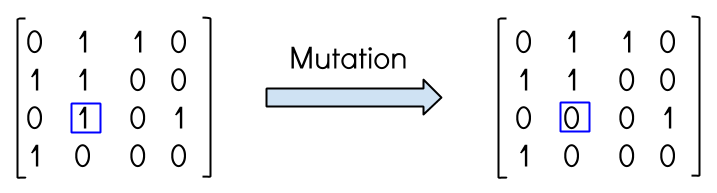
\includegraphics[width=0.5\textwidth]{pics/mutation.png}
\caption{Mutation}
\label{graph1}
\end{figure}

\begin{flushleft}\textbf{Crossover} This project adopt single point crossover. For each pair of chromosome, if a randomly generated number $rand < P_c$, where
$P_c$ is the crossover probability, then the crossover started.  Randomly choose a crossover point, and exchange the pieces from both chromosomes. Two offspring
are generated after this operation.
\end{flushleft}
                                   

\begin{figure}[!ht]
\centering
  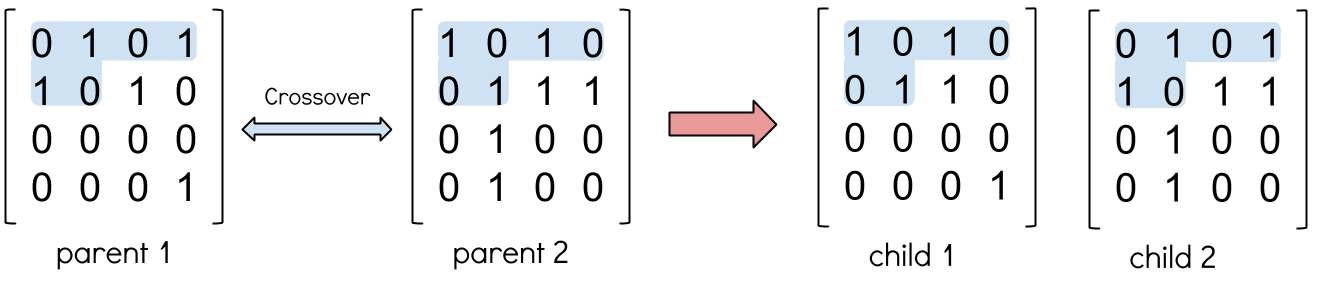
\includegraphics[width=0.7\textwidth]{pics/crossover.png}
\caption{Crossover}
\label{graph2}
\end{figure}

\subsection{Constraint Handling}
In Section \ref{C:single}, we defined the Web service location allocation problem with a single constraint. In order to fulfill the constraint,
we develop a repair function (Algorithm \ref{alg:repairfunctions}) to fix the invalid chromosomes. The reason that we use a repair function instead of
``death penalty'' is that ``death penalty'' is considered harmful in GA-based approaches. In GA-based approaches, chromosomes with bad fitness value
have large probability being removed from the population in the next generation. Hence, the algorithm would lose chance to search these areas. In contrast, 
in PSO-based approaches, particles with bad fitness value remain in the population. The invalid particles could move out of invalid regions in the next generation.
% The first function checks the Web service number constraint and fix the chromosome by randomly deploying a service to a candidate location.
The function checks the constraint and fix an invalid chromosome by randomly deploying a web service to a candidate location.

% The second function checks the total cost constraint and repeatly reduce the redundant deployment of service. If there is no redundant deployment but
% the cost limitation still can not be satisfied, the repair function would return the last repaired chromosome.

% The repair functions manually intervene the evolutionary process. The repair process also involves randomness. 


\begin{algorithm}[!h]
	\caption{Repair Algorithm}
	\footnotesize
	\label{alg:repair}
	\textbf{Inputs:} \\
		Population

	\textbf{Outputs:}
		A repaired population

	\begin{algorithmic}[1]
		\For( each chromosome)
		\While{ violate service number constraint}
		\State randomly choose a location $j$ and set $a_{sj}$ = 1
		\EndWhile
% 		
% 		\While{ violate cost constraint}
% 		\If ( no multiple services deployed in any locations $j$)
% 		  \State return with original chromosome
% 		\EndIf
% 		\State randomly cancel a deployment where there are multiple deployment in one location
% 		\EndWhile
% 		\EndFor
% 		\State Return the repaired population
	\end{algorithmic}
	\label{alg:repairfunctions}
\end{algorithm}





\section{Experiment Design}
We conduct experiments using the 14 problem cases described in Section \ref{sec:datasets} over three algorithms: BPSO (Algorithm \ref{alg:BPSO}), NSGA-II (Algorithm \ref{alg:NSGA2}) and NSPSO (Algorithm \ref{alg:NSPSO}). In order to assess and compare the quality of their solutions, 
hypervolume method \cite{Auger:2009} is applied. Hypervolume calculates the volume between the non-dominated curve with respective to a reference point ((1, 1) 
in this project). Hypervolume measures both diversity as well as convergence.

The parameters are shown in Table \ref{tab:para}. Specifically, we treat both objectives equally important, so the weight parameter $w$ in BPSO is set 
to 0.5. Each algorithm is conducted 40 runs to meet the statistical minimum requirements.

BPSO with an aggregating approach outputs a solution set without using a non-dominated sorting.  In order to compare
with other multi-objective algorithms, the non-dominated solutions are extracted from its output.

To show the performance of the three algorithms, we compare the \emph{best solutions} generated by the algorithm and the \emph{average solutions} generated
by the algorithms.  
A \emph{best solution} set is generated by applying fast non-dominated sorting over a combination of 40 runs of solutions. 
We compare different algorithms by plotting best solutions from algorithms.
In \emph{average solutions}, we apply hypervolume method 
on the solutions of 40 runs.
The mean and standard deviation of 40 hypervolume values are calculated.


\begin{table}[!h]
\centering
\footnotesize
\caption{Parameter Settings}
\label{tab:para}
\begin{tabular}{l|l|l|l|l|l|l|l}
\hline
Method                                                         & Population              & Maximum Iteration       & c1                                                                     & c2                                                                     & w                                                                      & $P_m$                                                                    & $P_c$                                                                    \\ \hline
\begin{tabular}[c]{@{}l@{}}BPSO\\ NSGA-II\\ NSPSO\end{tabular} & \multicolumn{1}{c|}{50} & \multicolumn{1}{c|}{50} & \multicolumn{1}{c|}{\begin{tabular}[c]{@{}c@{}}2\\ -\\ 2\end{tabular}} & \multicolumn{1}{c|}{\begin{tabular}[c]{@{}c@{}}2\\ -\\ 2\end{tabular}} & \multicolumn{1}{c|}{\begin{tabular}[c]{@{}c@{}}1\\ -\\ 1\end{tabular}} & \multicolumn{1}{c|}{\begin{tabular}[c]{@{}c@{}}-\\ 0.2\\ -\end{tabular}} & \multicolumn{1}{c}{\begin{tabular}[c]{@{}c@{}}-\\ 0.8\\ -\end{tabular}} \\ \hline
\end{tabular}
\end{table}


\section{Results}

\begin{table}[!h]
\centering
\footnotesize
\caption{Comparison between NSPSO, NSGA-II and BPSO: The mean and standard deviation of the hypervolume values over the 40 independent runs}
\label{tab:threeresults}
\scalebox{0.9}{
\begin{subtable}{.5\linewidth}
\centering
\begin{tabular}{|c|l|c|c|}
\hline
Dataset                         & \multicolumn{1}{c|}{Method}                                              & Hypervolume (avg $\pm$ sd)                                                                                                     \\ \hline
problem 1                       & \begin{tabular}[c]{@{}l@{}}NSPSO\\ NSGA-II\\ BPSO\end{tabular} & \begin{tabular}[c]{@{}c@{}} 0.76 $\pm$ 0.019\\ 0.83 $\pm$ 0.013\\ \textbf{0.89 $\pm$ 0.016}\end{tabular}  \\ \hline
problem 2                       & \begin{tabular}[c]{@{}l@{}}NSPSO\\ NSGA-II\\ BPSO\end{tabular} & \begin{tabular}[c]{@{}c@{}} \textbf{0.61 $\pm$ 0.011}\\ 0.60 $\pm$ 0.012\\  \textbf{0.61}$\pm$ 0.01\end{tabular} \\ \hline
problem 3                       & \begin{tabular}[c]{@{}l@{}}NSPSO\\ NSGA-II\\ BPSO\end{tabular} & \begin{tabular}[c]{@{}c@{}} 0.61 $\pm$ 0.011\\ 0.59 $\pm$ 0.007\\ \textbf{0.69 $\pm$ 0.007}\end{tabular}  \\ \hline
problem 4                       & \begin{tabular}[c]{@{}l@{}}NSPSO\\ NSGA-II\\ BPSO\end{tabular} & \begin{tabular}[c]{@{}c@{}} 0.63 $\pm$ 0.011\\ 0.61 $\pm$ 0.007\\ \textbf{0.71 $\pm$ 0.008}\end{tabular}  \\ \hline
problem 5                       & \begin{tabular}[c]{@{}l@{}}NSPSO\\ NSGA-II\\ BPSO\end{tabular} & \begin{tabular}[c]{@{}c@{}} 0.61 $\pm$ 0.009\\ 0.58 $\pm$ 0.005\\ \textbf{0.67 $\pm$ 0.007}\end{tabular}  \\ \hline
\multicolumn{1}{|l|}{problem 6} & \begin{tabular}[c]{@{}l@{}}NSPSO\\ NSGA-II\\ BPSO\end{tabular} & \begin{tabular}[c]{@{}c@{}} 0.59 $\pm$ 0.007\\ 0.55 $\pm$ 0.006\\ \textbf{0.63 $\pm$ 0.005}\end{tabular}  \\ \hline
problem 7                       & \begin{tabular}[c]{@{}l@{}}NSPSO\\ NSGA-II\\ BPSO\end{tabular} & \begin{tabular}[c]{@{}c@{}} 0.60 $\pm$ 0.008\\ 0.56 $\pm$ 0.005\\ \textbf{0.63 $\pm$ 0.006}\end{tabular}  \\ \hline
\end{tabular}
\end{subtable}

\begin{subtable}{.5\linewidth}
\centering
\begin{tabular}{|c|l|c|c|}
\hline
Dataset                         & \multicolumn{1}{c|}{Method}                                              & Hypervolume (avg $\pm$ sd)                                                                                                    \\ \hline
problem 8                       & \begin{tabular}[c]{@{}l@{}}NSPSO\\ NSGA-II\\ BPSO\end{tabular} & \begin{tabular}[c]{@{}c@{}} 0.61 $\pm$ 0.008\\ 0.58 $\pm$ 0.005\\ \textbf{0.65 $\pm$ 0.008}\end{tabular}  \\ \hline
problem 9                       & \begin{tabular}[c]{@{}l@{}}NSPSO\\ NSGA-II\\ BPSO\end{tabular} & \begin{tabular}[c]{@{}c@{}} 0.60 $\pm$ 0.009\\ 0.56 $\pm$ 0.004\\ \textbf{0.62 $\pm$ 0.005}\end{tabular}  \\ \hline
problem 10                      & \begin{tabular}[c]{@{}l@{}}NSPSO\\ NSGA-II\\ BPSO\end{tabular} & \begin{tabular}[c]{@{}c@{}} 0.58 $\pm$ 0.008\\ 0.53 $\pm$ 0.005\\ \textbf{0.58 $\pm$ 0.005}\end{tabular}  \\ \hline
problem 11                      & \begin{tabular}[c]{@{}l@{}}NSPSO\\ NSGA-II\\ BPSO\end{tabular} & \begin{tabular}[c]{@{}c@{}} \textbf{0.57 $\pm$ 0.009}\\ 0.52 $\pm$ 0.003\\ 0.55 $\pm$ 0.003\end{tabular} \\ \hline
problem 12                      & \begin{tabular}[c]{@{}l@{}}NSPSO\\ NSGA-II\\ BPSO\end{tabular} & \begin{tabular}[c]{@{}c@{}} \textbf{0.58 $\pm$ 0.009}\\ 0.52 $\pm$ 0.003\\ 0.56 $\pm$ 0.003\end{tabular} \\ \hline
problem 13                      & \begin{tabular}[c]{@{}l@{}}NSPSO\\ NSGA-II\\ BPSO\end{tabular} & \begin{tabular}[c]{@{}c@{}} \textbf{0.59 $\pm$ 0.008}\\ 0.53 $\pm$ 0.003\\ 0.56 $\pm$ 0.004\end{tabular} \\ \hline
problem 14                      & \begin{tabular}[c]{@{}l@{}}NSPSO\\ NSGA-II\\ BPSO\end{tabular} & \begin{tabular}[c]{@{}c@{}} \textbf{0.59 $\pm$ 0.009}\\ 0.53 $\pm$ 0.002\\ 0.57 $\pm$ 0.003\end{tabular} \\ \hline
\end{tabular}
\end{subtable}
}
\label{tab:ave}
\end{table}

\begin{figure}[t]
  \caption{NSPSO, NSGA-II and BPSO Experiments: The non-dominated solutions among the set obtained by 40 independent runs}
   \centering
   \begin{subfigure}{0.30\textwidth}
       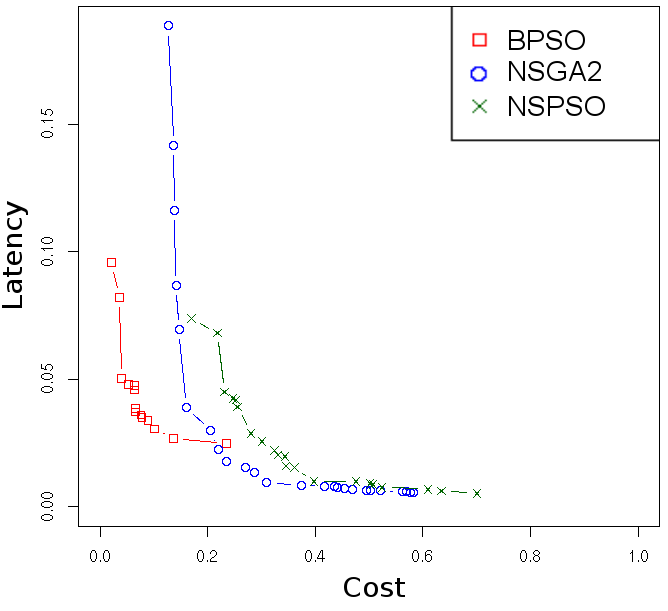
\includegraphics[width=\textwidth]{pics/nsgabpso1.png}
	   \caption{Problem 1}
   \end{subfigure}
   \begin{subfigure}{0.30\textwidth}
       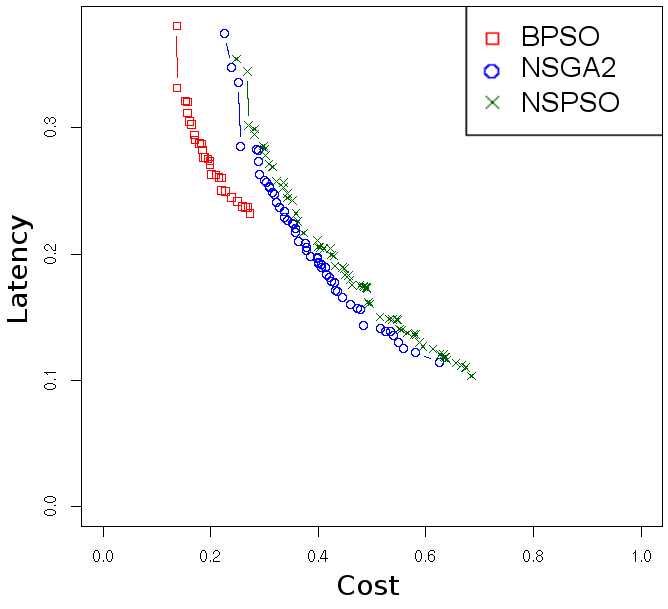
\includegraphics[width=\textwidth]{pics/nsgabpso2.png}
	   \caption{Problem 2}
   \end{subfigure}
   \begin{subfigure}{0.30\textwidth}
       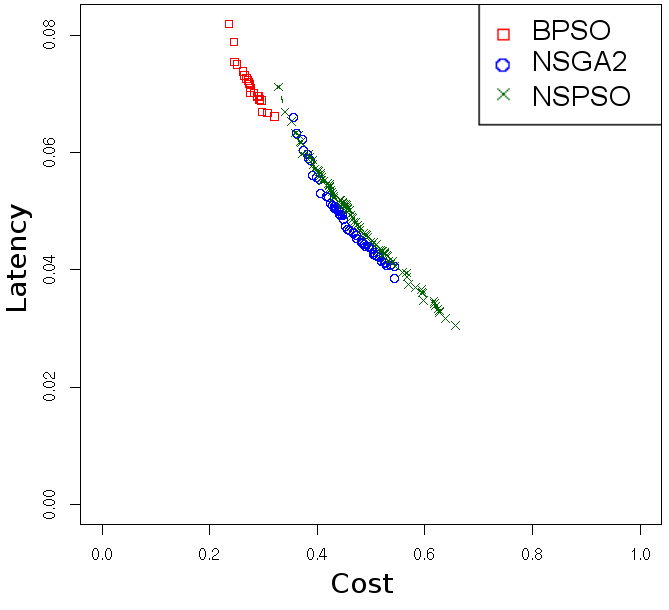
\includegraphics[width=\textwidth]{pics/nsgabpso3.png}
	   \caption{Problem 3}
   \end{subfigure}
      \begin{subfigure}{0.30\textwidth}
       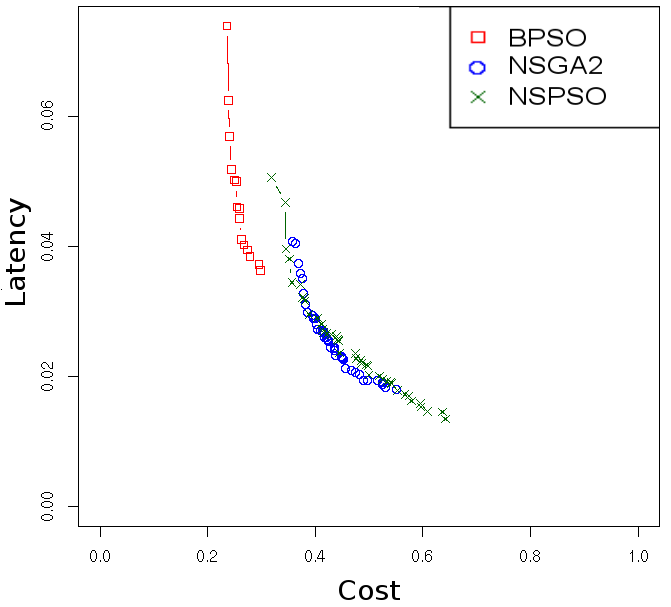
\includegraphics[width=\textwidth]{pics/nsgabpso4.png}
	   \caption{Problem 4}
   \end{subfigure}
      \begin{subfigure}{0.30\textwidth}
       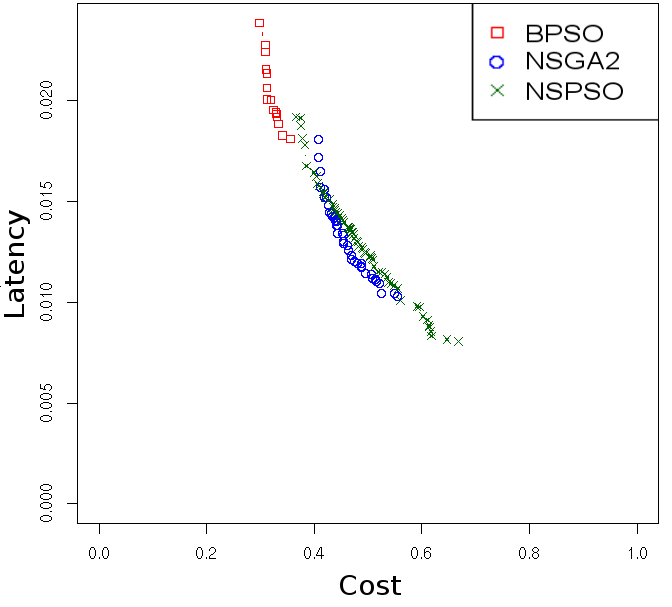
\includegraphics[width=\textwidth]{pics/nsgabpso5.png}
	   \caption{Problem 5}
   \end{subfigure}
   \begin{subfigure}{0.30\textwidth}
       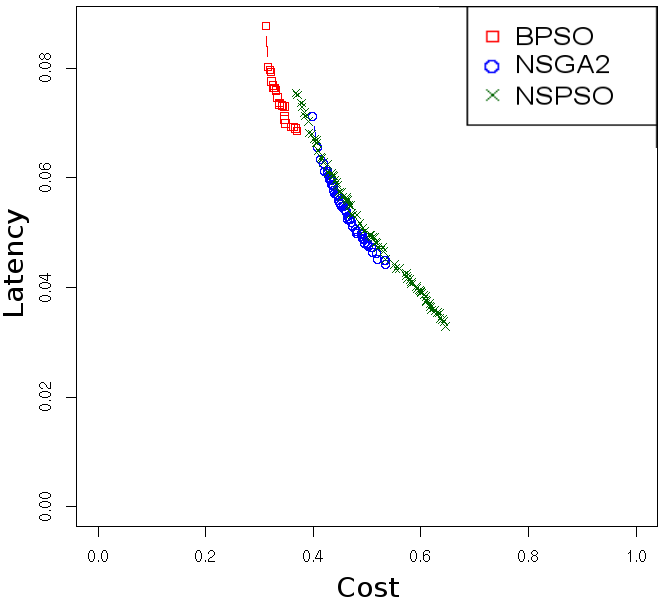
\includegraphics[width=\textwidth]{pics/nsgabpso6.png}
	   \caption{Problem 6}
   \end{subfigure}
   \begin{subfigure}{0.30\textwidth}
       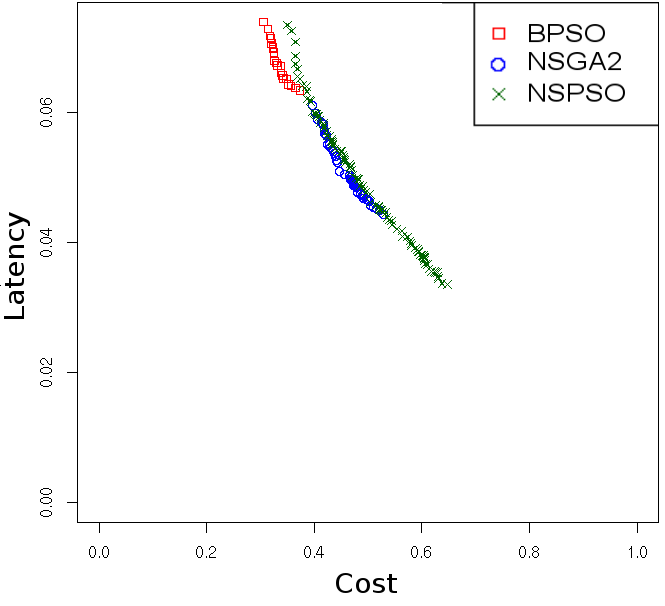
\includegraphics[width=\textwidth]{pics/nsgabpso7.png}
	   \caption{Problem 7}
   \end{subfigure}
      \begin{subfigure}{0.30\textwidth}
       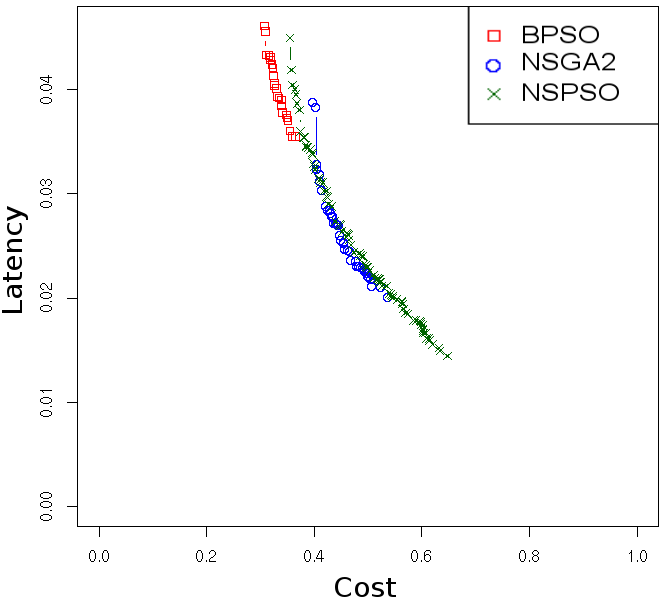
\includegraphics[width=\textwidth]{pics/nsgabpso8.png}
	   \caption{Problem 8}
   \end{subfigure}
      \begin{subfigure}{0.30\textwidth}
       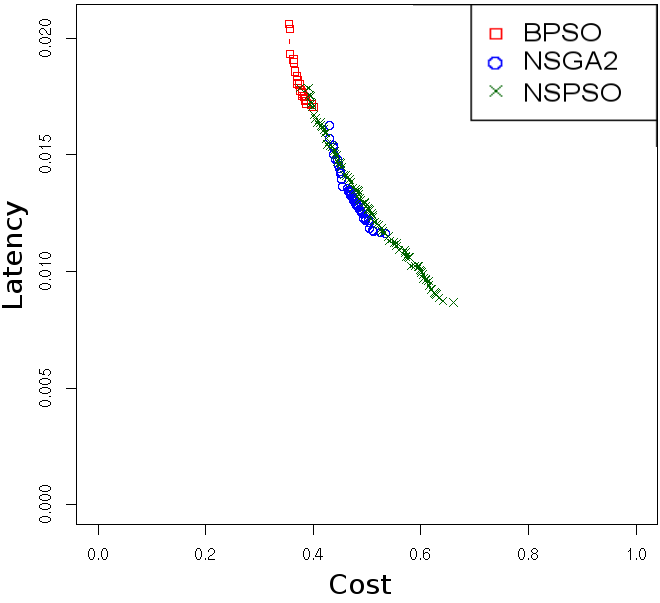
\includegraphics[width=\textwidth]{pics/nsgabpso9.png}
	   \caption{Problem 9}
   \end{subfigure}
   \begin{subfigure}{0.30\textwidth}
       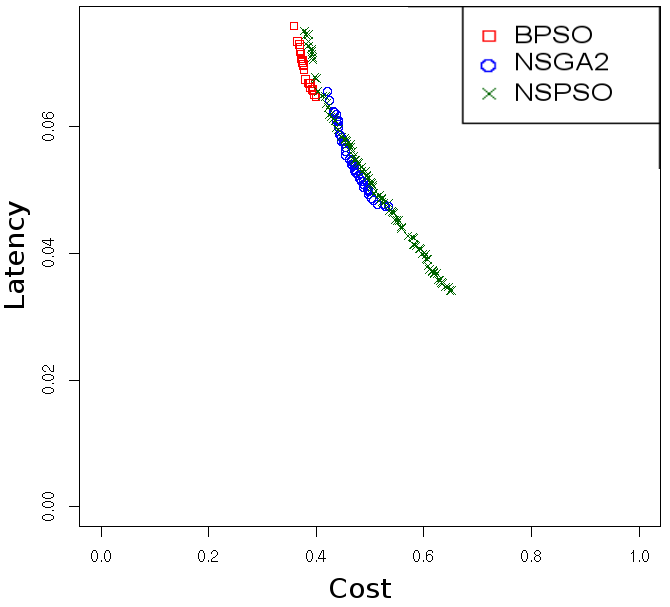
\includegraphics[width=\textwidth]{pics/nsgabpso10.png}
	   \caption{Problem 10}
   \end{subfigure}
   \begin{subfigure}{0.30\textwidth}
       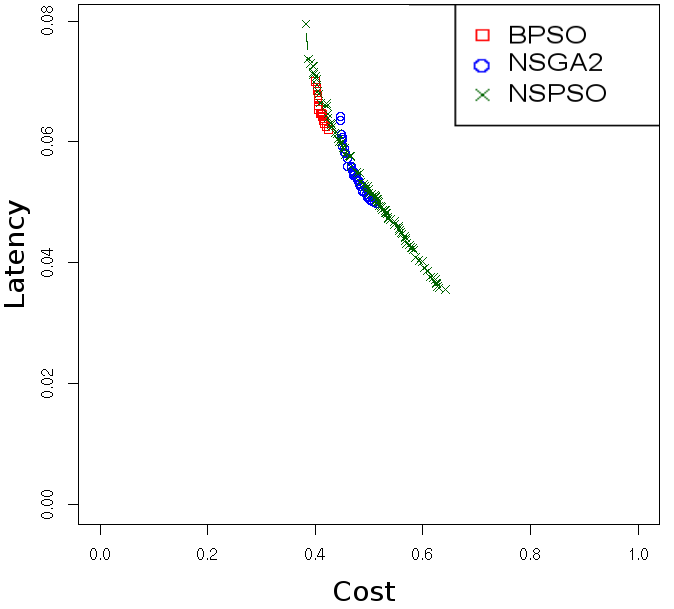
\includegraphics[width=\textwidth]{pics/nsgabpso11.png}
	   \caption{Problem 11}
   \end{subfigure}
   \begin{subfigure}{0.30\textwidth}
       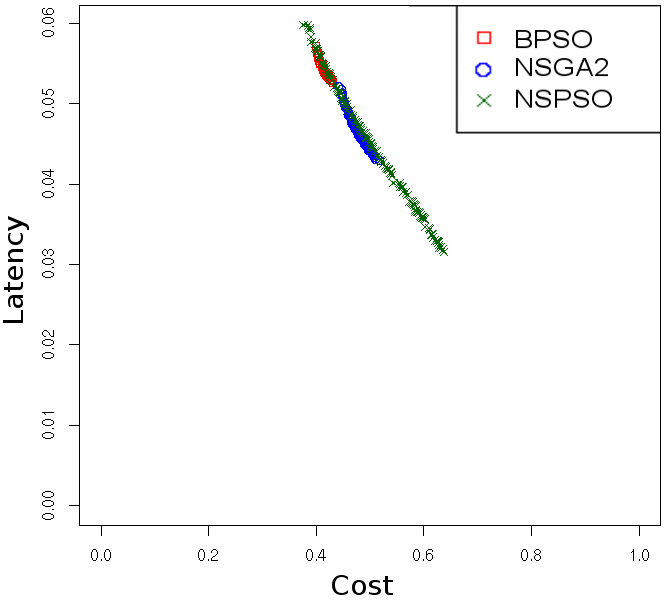
\includegraphics[width=\textwidth]{pics/nsgabpso12.png}
	   \caption{Problem 12}
   \end{subfigure}
      \begin{subfigure}{0.30\textwidth}
       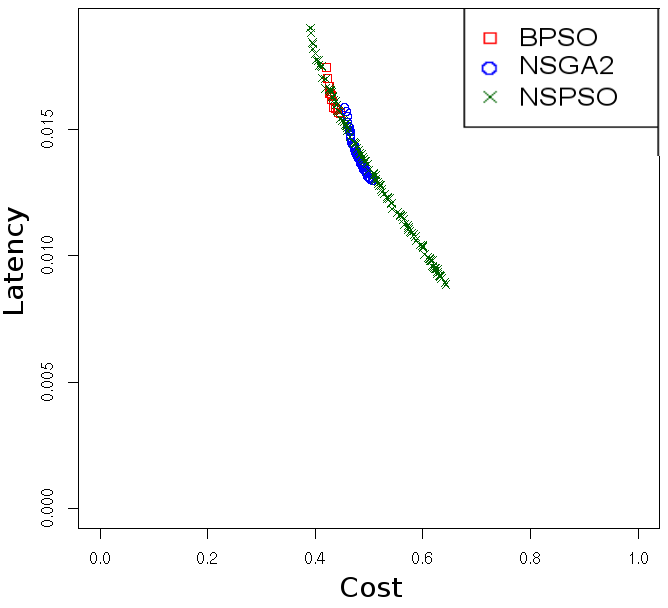
\includegraphics[width=\textwidth]{pics/nsgabpso13.png}
	   \caption{Problem 13}
   \end{subfigure}
      \begin{subfigure}{0.30\textwidth}
       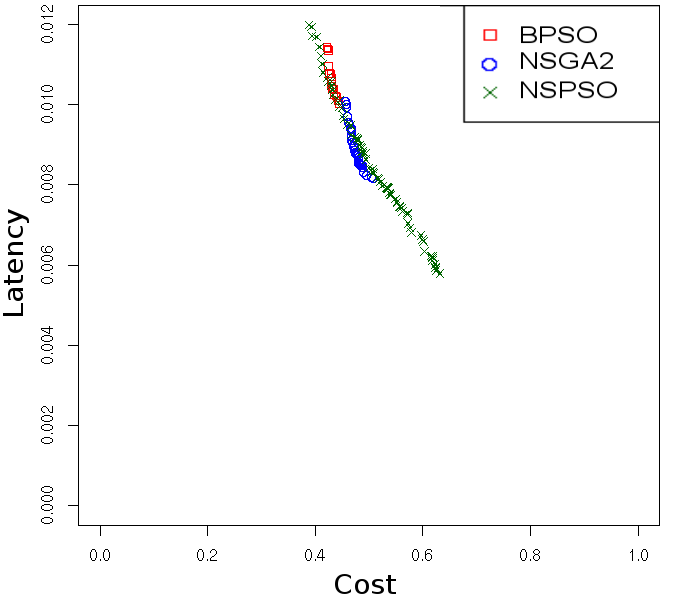
\includegraphics[width=\textwidth]{pics/nsgabpso14.png}
	   \caption{Problem 14}
   \end{subfigure}
   \label{fig:nsgabpso}
\end{figure}

The \emph{average solutions} are shown in Table \ref{tab:ave}. The \emph{best solutions} are shown in Figure \ref{fig:nsgabpso}.
In \emph{average solutions}, BPSO dominates the other two algorithms in the first ten problems. In the last four problems, 
NSPSO dominates the performance. 
In the \emph{best solutions}, 
it shows the solutions from BPSO has better convergence for the first two problems as they are closer to the original point. As the problem size getting larger,
BPSO's advantage of convergence gradually diminishes. 
In addition, the diversity of BPSO is clearly much worse than NSGA-II and NSPSO as its solutions could 
only cover a small region of the Pareto front.

In comparison between NSGA-II and NSPSO, NSPSO has a better performance in all problems except the first one (Table \ref{tab:threeresults}). NSPSO's advantage in diversity become more and more clear as the problem size increases.
In the first and second problem, NSGA-II dominates NSPSO in convergence. From problem 3, NSPSO outperforms
NSGA-II in both measurements. The diversity of solutions is the major difference between NSPSO and NSGA-II. 
Especially, when the data set is getting very large, NSPSO could still maintain a diverse of solutions while 
the other algorithms could only provide some solutions within a narrow area.

Another observation is that, there is a decreasing trend in the average solutions among all three algorithms with the problem size increasing.

\section{Discussions}
The experiments show that in terms of convergence, 
the performance of BPSO is better than NSPSO and NSGA-II in handling small problems. 
In terms of diversity, NSPSO has a big advantage in most cases.
There are two major problems that we noticed from the current results.
Firstly, the solutions are not diverse enough. Figure \ref{fig:nsgabpso}, especially, Problems 3 $\sim$ 9 show that NSPSO could not cover the Pareto front.
It is because NSPSO lacks a mechanism to avoid being stuck at local optima.
Secondly, all three algorithms are suffering from decreasing of performance when problem size increases. 
It is a major problem since the number of web services and locations are increasing everyday.
An algorithm without scalability would be less useful for service allocation task with a big search space.

\section{Summary}
In this chapter, we proposed a  NSPSO-based approach to solve the Web service location allocation with two fitness functions.
In order to show the quality of its solutions, we compare it with a NSGA-II approach.
We conducted experiments with the three algorithms over 14 problems.
The results show NSPSO provides diverse solutions in most cases. 
The results also show all three algorithms have poor performances when handling big datasets. 
In the next step, we are going to solve this problem by developing a new BMOPSOCD approach.

\chapter{A new BMOPSOCD for Service Location Allocation}
\label{C:bmopsocd}
\section{Introduction}
In the previous chapter, we find that there are two major shortcomings in BPSO, NSPSO and NSGA-II. The first one is
their performances drop rapidly when the dataset increases. The second shortcoming is that 
the solutions are not diverse enough. In order to further improve the performance, 
this chapter develops a new binary multi-objective PSO with crowding distance approach to solve the Web service location allocation problem. 
We introduce a new mechanism, the rounding function to the original MOPSOCD. The rounding function method is a mechanism
that makes a continuous algorithm compatible with discrete problems. 

We develop this approach based on MOPSOCD \cite{Raquel} because it has two desired features: archive and mutation. These features make the algorithm to have  a strong ability to avoid stucking at local optima while maintaining an 
uniformly non-dominated set. 



\section{BMOPSOCD}
The selection of $pbest$ and $gbest$ is one of the key steps in BMOPSOCD.
$pbest$ is the personal best solution of each particle in population. The $pbest$ is updated only if the new particle dominates the current one, otherwise it remains unchanged.

In the BMOPSOCD, any non-dominated solutions in the archive can be a $gbest$, therefore, it is important to ensure that the particles move to an unexplored area. The $gbest$ is selected from non-dominated solutions with highest crowding distance value. It ensures the swarm to move to a least crowded area.

\begin{algorithm}[!htb]
	\caption{BMOPSOCD for Web Service Location Allocation}
	\footnotesize
	\textbf{Inputs:} \\
		Cost Matrix $C$, \\
		Server network latency matrix $L$, \\
		Service invocation frequency matrix $F$ \\
	\textbf{Outputs:}
		Pareto Front: the $Archive$ set

	\begin{algorithmic}[1]
		\State Initialize a population $P$ with random real values $\in$ (0, 1)
		\State Initialize velocity[i] = 0
		\State \textbf{Each individual $i$ in $P$ using the rounding function and then applies fitness functions}
		\State Initialize personal best of each individual $i$.
		\State Initialize $GBEST$
		\State Initialize $Archive$ with non-dominated vectors found in $P$

		\Repeat
			\State Compute the crowding distance values of each non-dominated solution in the $Archive$
			\State Sort the non-dominated solutions in $Archive$ in descending crowding distance values
			\For ( each particle)
				\State Randomly select the global best guide for P[i] from a specified top portion of the sorted archive A and store its position to GBEST.
				\State Compute the new velocity 
				\State Update its position
				\State If it goes beyond the boundaries, then multiply its velocity by -1
				\State If($t < (MAXT * PMUT)$), apply Mutation
				\State Rounding and evaluating fitness
				\State Update its $PBESTS$
				\EndFor
		\State Insert new non-dominated solution into $Archive$, remove dominated solutions from $Archive$
		\Until{ maximum iterations is reached}
		\State return $Archive$
	\end{algorithmic}
	\label{alg:BMOPSOCD}
\end{algorithm}

\subsection{Particle Representation}
The major difference between BMOPSOCD and the other three algorithms is the particle representation. 
Although it is a binary approach, the particle remains a continuous representation.
We also employ the flatten method as described in the previous section.

 \begin{figure}[H]
 \centering
   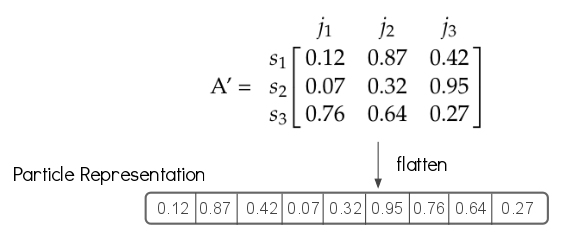
\includegraphics[width=0.7\textwidth]{pics/flatten.png}
   \caption{BMOPSOCD particle representation}
   \label{fig:flatten}
 \end{figure}

\subsection{Fitness Function}
Two fitness functions are used to achieve two objectives, cost fitness and latency fitness.
They are the same for NSPSO, defined in Section \ref{sec:nspsofitness}.



\subsection{Constraint Handling}

The constraint handling method used by BMOPSOCD is a ranking of violations. 
A solution $I$ is considered to constraint-dominate a solution $J$ if any of the following conditions is true:
\begin{enumerate}
 \item Solution $I$ is feasible, solution $J$ is not,
 \item Both solutions are infeasible, solution $I$ has less violations,
 \item Both solutions are feasible, solution $I$ dominates solution $J$.
\end{enumerate}

The particle with less violations is always considered as  a better solution. 
If there is only one constraint, this constraint handling method provides similar effect with death penalty method.


\subsection{Rounding Functions}

The original MOPSOCD is designed as a continuous version PSO. Instead of changing the particle to a binary representation, we still use the continuous representation. 
In order to be compatible with the binary problem, the continuous representation particle needs
to be transformed to a binary representation during the evaluation of fitness.
That is, in the initial stage, particles are initialized in real values. The updates of velocity and position are as usual. 
During the evaluation of fitness, the first step is to transform the real representation particle to binary. Then, evaluate the binary particle using
the fitness functions.

The rounding function is used to map a real value particle to a discrete value particle.
The common strategy is to round a real value to its closest integer number.
The round-down strategy is adopted in \cite{1004478} to solve integer programming problem. 
\cite{4120263} uses a real value representation of chromosome for GA. 
Then the real value chromosome is rounded to integer and binary representations in order to 
achieve a mixed integer optimization of array antenna pattern and micro-strip antenna. 
\cite{liu2013discrete} adopts rounding and interval mapping strategy to solve 0-1 discrete,
integer optimization and mixed optimization problem. 
\cite{Anghinolfi200973} uses a random-round function which randomly returns round-up value or round-down value.

\subsubsection{A Static Rounding Function}

A static rounding function is a straightforward strategy. A parameter threshold $t$ is introduced in the static rounding function.
The value of a particle entry is either round up or round down according to $t$. 
The threshold value $t$ is rather ad-hoc that based on empirical study.
 \begin{equation}
 	\label{eq:1}
 	a_{sj} = 
 	\begin{cases}
 		1 & \quad \text{if } a'_{sj} > t \\
 		0 & \quad \text{otherwise} \\
 	\end{cases}
 \end{equation}

 
\subsubsection{Dynamic Rounding Functions}
\label{sec:dynamic}
The threshold plays an important role in constraining the particle swarm in the search space.
The static rounding function has the following drawbacks. Firstly, the parameter threshold $t$ needs to be predefined. 
The value of threshold $t$ is problem specific, therefore, it is hard to estimate the performance before obtaining the results.
Secondly, the influence of different threshold values are not completely studied. Because of the above reasons, a dynamic rounding threshold
is proposed. A dynamic rounding function has two steps. In the first step, it adjusts the value of threshold $t$ according to the current generation. 
The second step is the same as static rounding function, either round up or round down according to $t$. Three dynamic rounding functions are considered. Equation \ref{eq:linear} is a linear function.
Equation \ref{eq:quadratic} is a quadratic function. Equation \ref{eq:reciprocal} is a reciprocal function. The reason that we design three 
dynamic functions is that we would like to compare the impact of different trajectories of dynamic thresholds.
$t$ is the value of threshold, $g$ is the current generation. The lower boundary of a threshold is $l$, upper boundary is $u$.
They are predefined.
The performance of these rounding functions is studied in the Section \ref{sec:expdy}.

\begin{equation}
\label{eq:linear}
 t = \frac{l - u}{\text{max generation}} g + u
\end{equation}

\begin{equation}
\label{eq:quadratic}
 t = \frac{l - u}{(\text{max generation})^2} g^2 + u
\end{equation}

\begin{equation}
\label{eq:reciprocal}
 t = u - \frac{u - l}{\text{max generation} - g}  (g \neq \text{max generation})
\end{equation}

% The rounding process can be done in fitness function so that there is no need to modify the PSO.

% We introduced a \emph{service location-allocation probability matrix}, $A' = [a'_{sj}]$ represents the probability of a 
% service $s_{i}$ allocate to a candidate location $j_{i}$. 
% $a'_{sj}$ is a real value, $a'_{sj} \in (0, 1)$ indicate the probability of a service is \textbf{NOT} 
% allocate to a candidate location.
% 
% We use the service location-allocation probability matrix $A'$ = $[a'_{sj}]$ as a particle. 
% During the PSO process, the particle needs to be transfered to binary representation in order to compatible with 
% the modeling. In order to transfer $A' \rightarrow A$, we introduced a transformation
% function.
% 
\begin{figure}[H]
\centering
  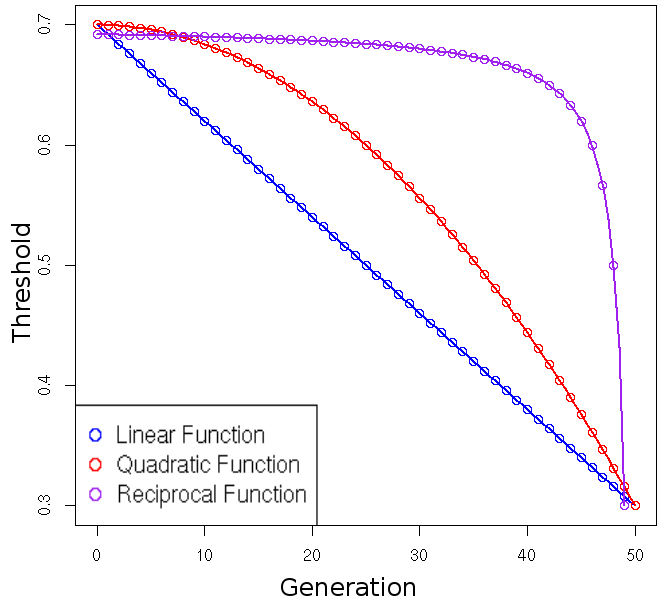
\includegraphics[width=0.5\textwidth]{pics/dynamic.png}
  \caption{Curve of three dynamic thresholds}
  \label{fig:dynamic}
\end{figure}
% 
% The parameter $threshold$ is an empirical parameter that introduced into the algorithm. 
\subsection{An Adaptive Threshold Approach}
\label{sec:transfer}
% As the problem becomes getting larger and larger, the performance of evolutionary computation drops. 
Human have the ability to learn a technique or knowledge and apply in different fields. 
As the dimensionality of the problem increases, the performance of evolutionary computation drops. 
It is necessary to build a system that has the ability to reuse the learned knowledge. 
Transfer learning is a process to reuse the knowledge in solving unseen tasks \cite{olivas}. 
In this section, we proposed an adaptive threshold that embodied in the transfer learning process.

Figure \ref{fig:adaptive} shows the evolutionary process with an adaptive threshold.
% The idea of transfer learning is inspired by \cite{Verbancsics}. 
Initially, the threshold $t$ is set to a upper boundary $u$ (e.g. 0.7). Then the PSO runns with this setting for a 
predefined interval $i$ (e.g. 10 generations). In the beginning of next interval (e.g. 11 generation), the threshold $t$ is changed according to
a function (Equation \ref{eq:transfer}) and remain steadily until next interval. 
Repeat this process until the lower boundary $l$ reached. 
The optimization may look like forcing the swarm ``jump'' to a different area. But the process is equivalent to initializing a new set of population with 
the old one. Therefore the knowledge are inherited.
An underlying assumption
is that, if the particle swarm could converge within an interval $i$, then it is better to explore a different direction.
Therefore, in the next interval, the swarm will explore a different area and is directed by an adjacent threshold value. 
The potential problem of the method is that it is hard to know whether the PSO is converged.
The transfer learning rounding function is shown in Equation \ref{eq:transfer} where $t'$ denotes the current threshold value.
\begin{figure}[H]
 \centering
   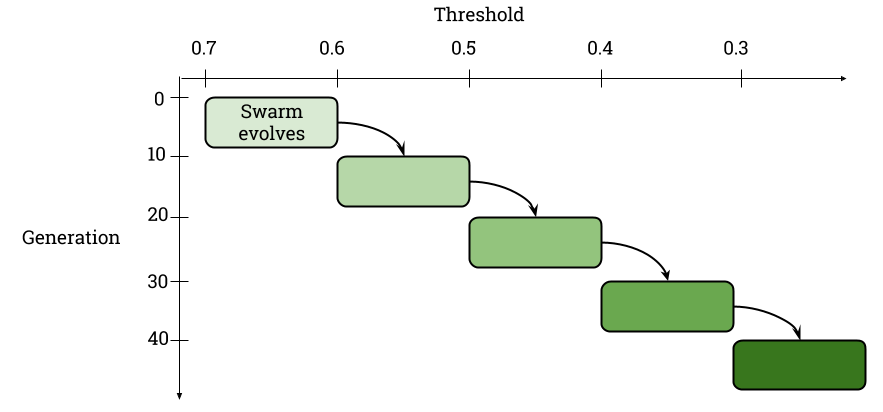
\includegraphics[width=0.7\textwidth]{pics/transfer.png}
   \caption{Evolutionary process with an adaptive threshold}
   \label{fig:adaptive}
 \end{figure}
 
\begin{equation}
\label{eq:transfer}
		t = 
		\begin{cases}
		= t' - \frac{u - l}{(\frac{\text{max generation}}{i} - 1)} & \quad \text{if } (\text{current generation}\mod i) = 0\\
		= t' & \quad \text{otherwise} \\
		\end{cases}
\end{equation}


\section{Experiment Design}
\label{sec:exp}
A set of experiments have been conducted over three major features of the proposal algorithm. 
The first feature considers the static threshold. The influence of the selection of 
different values of static threshold are studied in the first experiment. 
The second feature considers the dynamic rounding functions. Three different types of 
rounding function are examined in the second experiment. The third feature is the adaptive threshold. Its performance is studied in the third experiment. An experiment of a combination of static rounding function is conducted and discussed. Lastly, we conduct an experiment 
considering the overall performance of a BMOPSOCD with a dynamic rounding function in comparison with other three algorithms: PSO, NSPSO and NSGA-II (presented in Chapter \ref{C:multi}).



\subsection{Performance Metrics}
The IGD \cite{1501598} is a modified version of generational distance \cite{veldhuizen99, 870296} as a way of estimating 
how far the elements in the true Pareto front are from those in the Pareto front produced by our algorithm. 
It calculates the sum of the distances from each point of the true Pareto front to the nearest point of the non-dominated set that produced by an algorithm.
The lower the IGD, the better quality the solution is.
A true Pareto front is needed when calculating the IGD value.
For our problem, the true Pareto front is unknown, therefore, a approximated true Pareto front is produced by combining all the solutions produced by
4 algorithms (BMOPSOCD, NSGA-II, NSPSO, BPSO) and then apply a non-dominated sorting over it. The approximated true Pareto front dominates all the other solutions.
We use hypervolume and IGD as the evaluation metrics.

\subsection{Experiments on Rounding Functions}
This section designs four experiments to study the effect of different types of rounding functions. Four datasets (Problems 2 $\sim$ 5) are used, chosen from the Table \ref{tab:problem}. 

% The cost constraint is not considered in these experiments since it is not the study priority.
% The repair function of NSGA-II will also only use the Web service number constraint.

\subsubsection{Static Rounding Function}
\label{sec:static_exp}
There are two questions that we would like to answer with this experiment. 
The first question is what the influence of the threshold is. The second question is how to select a proper static threshold. 

In order to answer these two questions, a set of experiments is conducted using different static threshold values to evaluate the performance of 
the proposed algorithm.
The threshold value is ranged from 0.3 to 0.7.  
The parameters of the algorithm are set as follow, $w$ = 0.4, mutation probability $P_m$ = 0.5, $c1$ = 1, $c2$ = 1, archive size is 250, population size is  50 and
the max number of iteration is 50. For each experiment, the proposed algorithm has been independently run 40 times. 
The results are compared using the \emph{best result} approach. To obtain the \emph{best result} of 40 runs, the results of all 40 runs are combined, 
then a fast non-dominated sorting is applied over the combined results. 
\subsubsection{Dynamic Rounding Function}
In Section \ref{sec:dynamic}, three dynamic rounding functions are proposed. 
The performances of different rounding functions are the main purpose of the experiment. One major question is which dynamic rounding function provides the 
best results.
The parameters of the PSO algorithms are set as follows: $w$ = 0.4, mutation probability $P_m$ = 0.5, $c1$ = 1, $c2$ = 1, archive size is 250, 
population size is 50 and
the max number of iteration is 50. The upper boundary of dynamic threshold $u$ = 0.7 and the lower boundary of dynamic threshold $l$ = 0.3. 
The results are compared using \emph{average solutions}.

Figure \ref{fig:dynamic} shows threshold $t$ changes along with the generations. It is easy to notice that the points on linear and quadratic functions are 
uniformly distributed. Points on reciprocal are unevenly distributed.

\subsubsection{An Adaptive Threshold Approach}
The performance of the adaptive threshold approach is studied in this experiment.
The parameters of the PSO algorithms are set as follows: $w$ = 0.4, mutation probability $P_m$ = 0.5, $c1$ = 1, $c2$ = 1, archive size is 250, 
population size is 50 and
the max number of iteration is 50. The upper boundary of dynamic threshold $u$ = 0.7 and the lower boundary of dynamic threshold $l$ = 0.3. 
The interval is set to 10. The results are compared with dynamic functions with \emph{average solution} approach.



\subsubsection{A Combination of Static Rounding Function}
In the Section \ref{sec:static_exp}, we design an experiment to discover the effect of static thresholds. The idea of combination of static rounding funtion
is based on that experiment. The idea is obtaining the result produced by different thresholds and combining them into a dataset. Finally, 
employs a fast non-dominated sorting over the it. The experimental settings are the same as in Section \ref{sec:static_exp} and the result is 
evaluated with hypervolume and compared with reciprocal dynamic rounding.

\subsection{BMOPSOCD versus NSPSO, NSGA-II and BPSO}

In this section, we compare the performance of BMOPSOCD with other three algorithms.

The common parameter settings are shown in Table \ref{tab:settings}.
Specifically, we apply quadratic dynamic rounding function with [0.3, 0.7] boundaries in BMOPSOCD. The archive size is 250.
The results are compared using hypervolume and IGD. 
\begin{table}[H]
\centering
\footnotesize
\caption{Parameters}
\label{tab:settings}
\begin{tabular}{l|l|l|l|l|l|l|l}
\hline
Method                                                                   & Population              & Maximum Iteration       & c1                                                                         & c2                                                                         & w                                                                            & $P_m$                                                                          & $P_c$                                                                        \\ \hline
\begin{tabular}[c]{@{}l@{}}BMOPSOCD\\ NSPSO\\ NSGA-II\\ BPSO\end{tabular} & \multicolumn{1}{c|}{50} & \multicolumn{1}{c|}{50} & \multicolumn{1}{c|}{\begin{tabular}[c]{@{}c@{}}1\\ 2\\ -\\ 2\end{tabular}} & \multicolumn{1}{c|}{\begin{tabular}[c]{@{}c@{}}1\\ 2\\ -\\ 2\end{tabular}} & \multicolumn{1}{c|}{\begin{tabular}[c]{@{}c@{}}0.4\\ 1\\ -\\ 1\end{tabular}} & \multicolumn{1}{c|}{\begin{tabular}[c]{@{}c@{}}0.5\\ -\\ 0.2\\ -\end{tabular}} & \multicolumn{1}{c}{\begin{tabular}[c]{@{}c@{}}-\\ -\\ 0.8\\ -\end{tabular}} \\ \hline
\end{tabular}
\end{table}

We assume both objectives are equally important, therefore, a $weight$ for weighted-sum is set to 0.5. 
BPSO produces a bag of solution that is not a Pareto front. In order to compare BPSO with multi-objective algorithms, we first combine the solutions produced by 40 runs and then apply
fast non-dominated sorting to obtain a non-dominated solution set.




\section{Experimental Results and Discussion}
\subsection{Experiments on Rounding Functions}
\subsubsection{Static Rounding Function}

The experiment results of static threshold are shown in Figure \ref{fig:static}. It clearly show a pattern where the solution produced by different static thresholds
cover a part of the Pareto front but none of them is able to cover the complete Pareto front.

\begin{figure}[!h]
   \centering
   \begin{subfigure}{0.49\textwidth}
       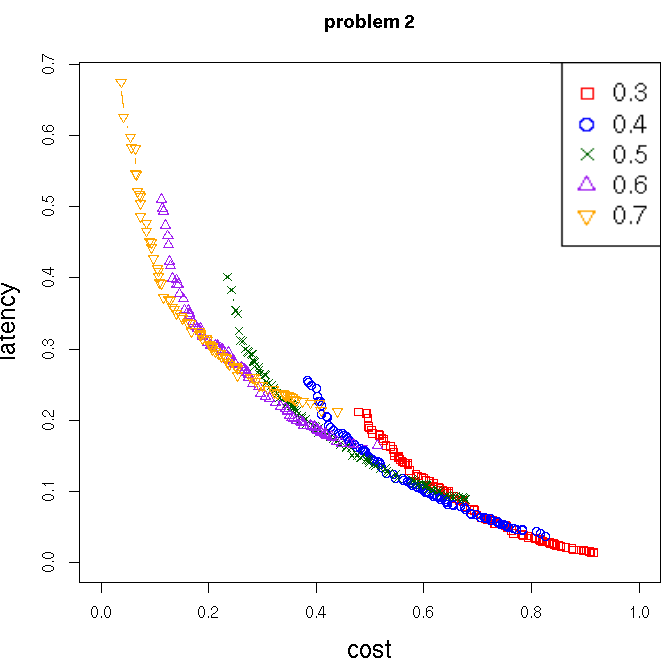
\includegraphics[width=\textwidth]{pics/static_threshold_problem_2.png}
	   \caption{}
   \end{subfigure}
   \begin{subfigure}{0.49\textwidth}
       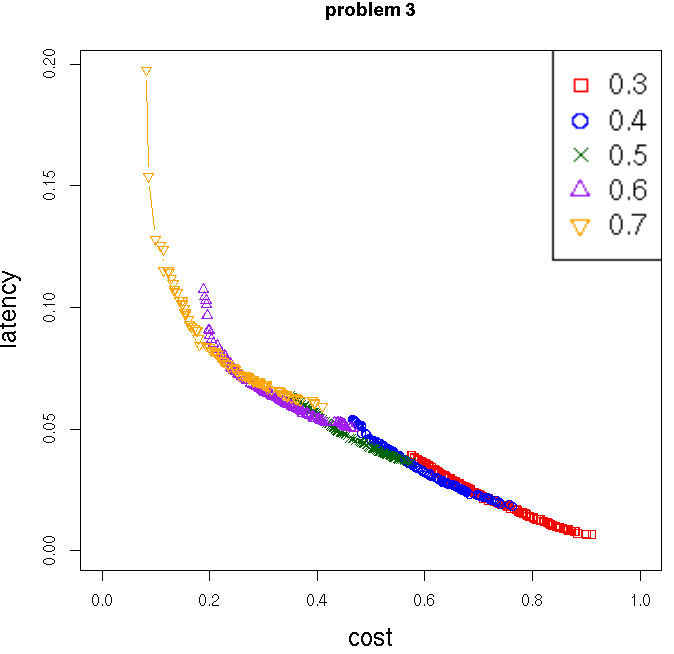
\includegraphics[width=\textwidth]{pics/static_threshold_problem_3.png}
	   \caption{}
   \end{subfigure}
   \begin{subfigure}{0.49\textwidth}
       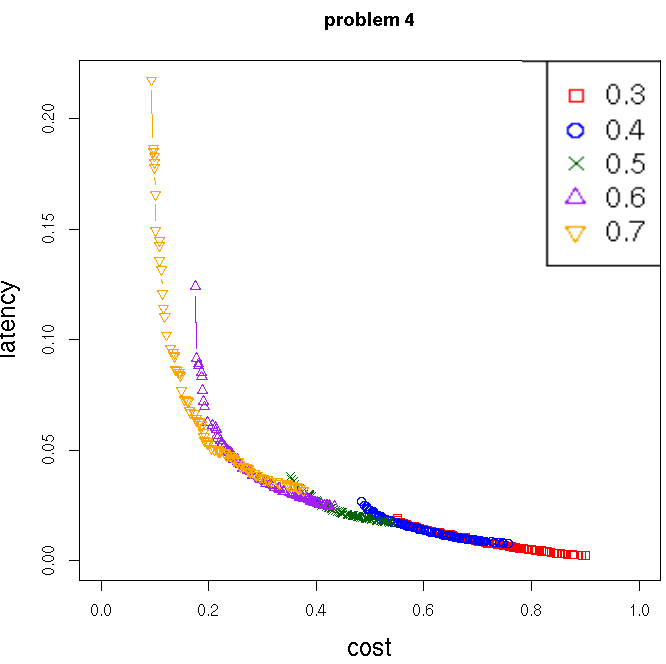
\includegraphics[width=\textwidth]{pics/static_threshold_problem_4.png}
	   \caption{}
   \end{subfigure}
   \begin{subfigure}{0.49\textwidth}
       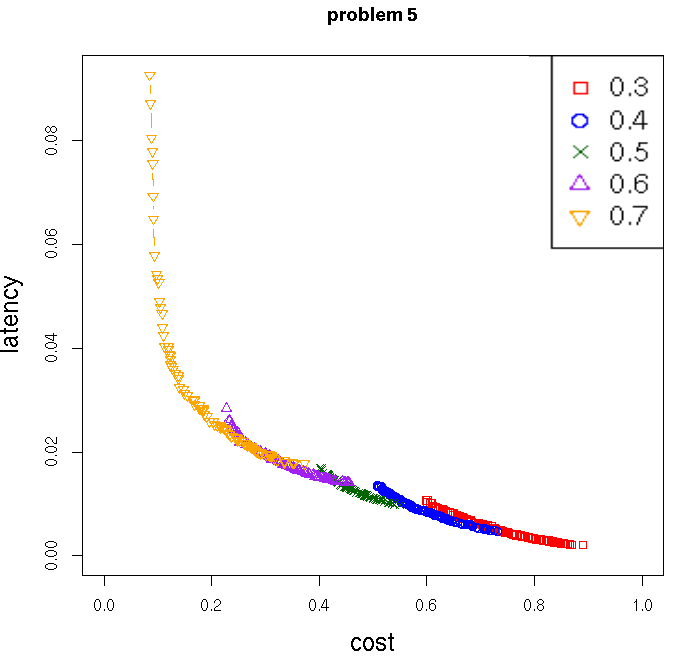
\includegraphics[width=\textwidth]{pics/static_threshold_problem_5.png}
	   \caption{}
   \end{subfigure}
   \caption{Static Rounding Function Experiments: Solutions from Problems 2 $\sim$ 5 with different static threshold values}
   \label{fig:static}
\end{figure}


The static threshold value has a huge impact of the final result. 
% Although the adjacent values are largely overlapped, none of them could cover the whole Pareto Front. 
The threshold value could ``clamp'' the  particle swarm to search a certain area. Take threshold value of 0.7 as an example (Figure \ref{fig:roundstatic}), 
when the rounding function rounds a real value to a binary value with respect the threshold 0.7, it means 70\% of probability 
rounds this value to 0. 

\begin{figure}[H]
\centering
  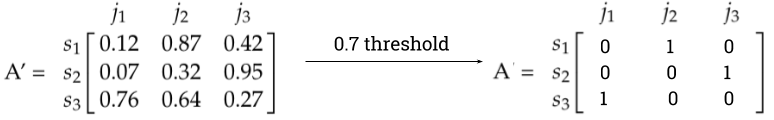
\includegraphics[width=0.7\textwidth]{pics/roundstatic.png}
  \caption{Rounding process}
  \label{fig:roundstatic}
\end{figure}

It means there are 70\% of chance avoid deploying a web service in a location. 
Intuitively, the optimization with threshold of 0.7 would considers optimizing cost over latency by deploying less web services. The swarm are under the 
direction of this ``savings'' policy. This effect is clearly shown on Figure \ref{fig:roundstatic}, where the solutions with 0.7 threshold 
scattered along the area with lower cost and higher latency. On the other hand, the solutions with $t< 0.5$ thresholds  are encouraged to optimize latency
over cost, therefore, more web services are deployed.

The experimental results clearly answered the first question: the influence of different thresholds. 
However, it is not offer a guide of selection of a proper threshold, because none of the solutions could cover the entire Pareto front.
Worth noting that, a solution of combining all results is ideal, as it largely improve the diversity of the non-dominated set. This observation inspires 
the development of dynamic threshold.

\subsubsection{Dynamic Rounding Functions}
\label{sec:expdy}
Table \ref{tab:hyperDynamic} shows the average performance of three dynamic functions that evaluated by hypervolume. 
The results indicate the reciprocal function dominated the three dynamic functions in all test cases. This effect could be visually observed by plotting the best results (Figure \ref{fig:dynamicFunctions}). 
Figure \ref{fig:dynamicFunctions} shows the reciprocal function slightly dominated the other two dynamic functions. 
However the problem of reciprocal function is that the solutions are not complete. There are gaps in Problems 3 $\sim$ 5. The gap is created because of the uniformity of the reciprocal function (Figure \ref{fig:dynamic}).

\begin{figure}[h!]
   \centering
   \begin{subfigure}{0.49\textwidth}
       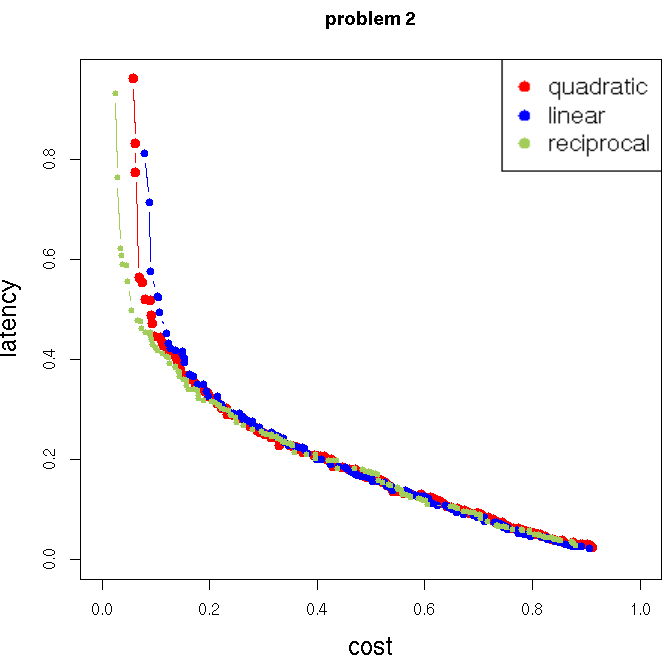
\includegraphics[width=\textwidth]{pics/dynamic_problem_2.png}
	   \caption{}
   \end{subfigure}
   \begin{subfigure}{0.49\textwidth}
       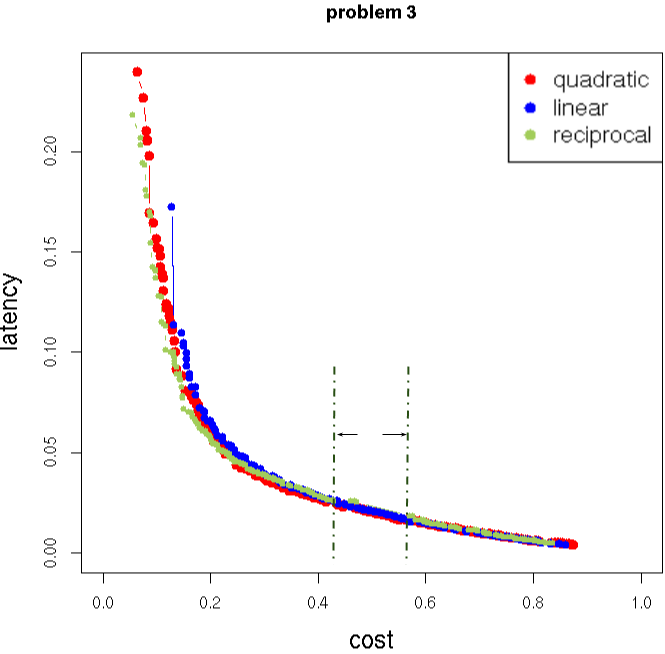
\includegraphics[width=\textwidth]{pics/dynamic_problem_3.png}
	   \caption{}
   \end{subfigure}
   \begin{subfigure}{0.49\textwidth}
       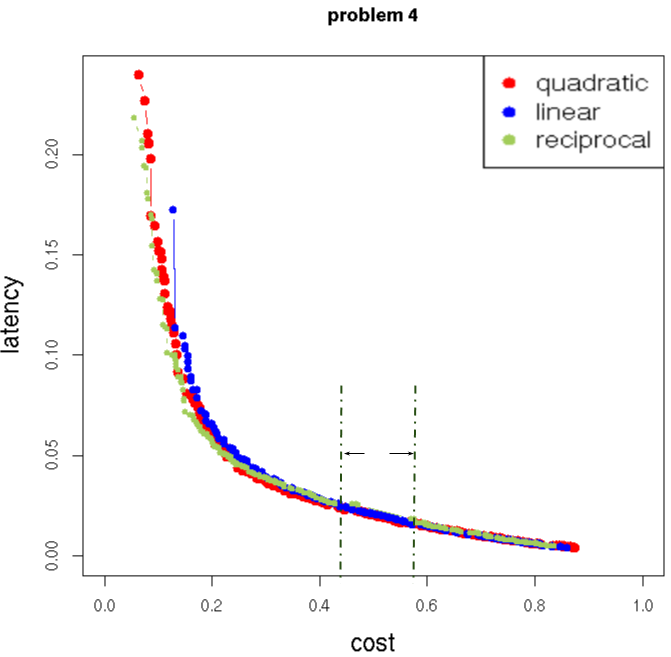
\includegraphics[width=\textwidth]{pics/dynamic_problem_4.png}
	   \caption{}
   \end{subfigure}
   \begin{subfigure}{0.49\textwidth}
       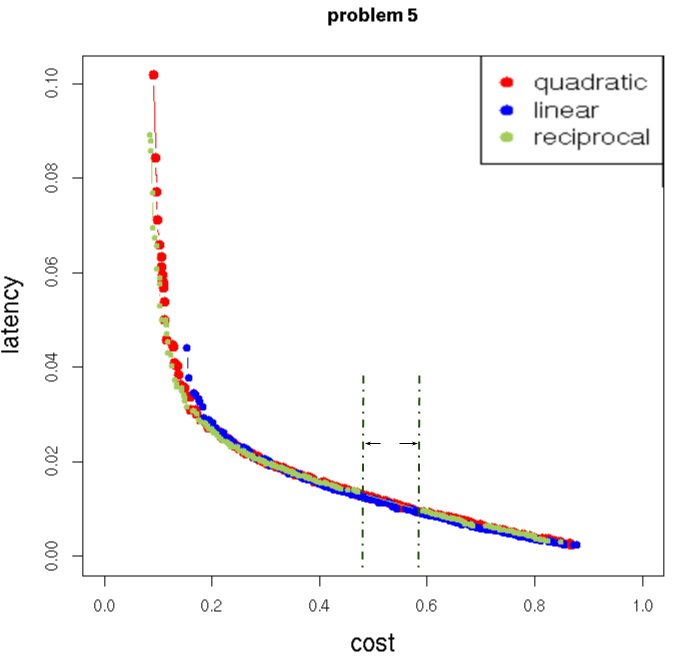
\includegraphics[width=\textwidth]{pics/dynamic_problem_5.png}
	   \caption{}
   \end{subfigure}
   \caption{Dynamic Rounding Function Experiments : The non-dominated solutions among the sets obtained by 40 independent runs of BMOPSOCD with different dynamic functions}
   \label{fig:dynamicFunctions}
\end{figure}


\begin{table}[H]
\centering
\footnotesize
\caption{The mean and standard deviation of the hypervolume values over the 40 independent runs}
\label{tab:hyperDynamic}
\begin{tabular}{l|c|c|c}
\hline
          & \multicolumn{1}{l|}{Linear} & \multicolumn{1}{l|}{Quadratic} & \multicolumn{1}{l}{Reciprocal}  \\ \hline
problem 2 & 0.72 $\pm$ 0.011            & 0.73 $\pm$ 0.008               & \textbf{0.74 $\pm$ 0.013}  	 \\ 
problem 3 & 0.80 $\pm$ 0.012            & 0.81 $\pm$ 0.012               & \textbf{0.815 $\pm$ 0.013}  		\\ 
problem 4 & 0.82 $\pm$ 0.012            & 0.86 $\pm$ 0.016               & \textbf{0.87 $\pm$ 0.014}  	\\ 
problem 5 & 0.80 $\pm$ 0.014            & 0.85 $\pm$ 0.023               & \textbf{0.86 $\pm$ 0.020}  	\\ \hline
\end{tabular}
\end{table}

According to Table \ref{tab:hyperDynamic}, the experimental results show that in terms of convergence, reciprocal function produces the best result. 
However, it also shows the major disadvantage of reciprocal function, which can not produce an entire Pareto front. In contrast, quadratic function performs
a little worse in convergence but obtains an uniformly distributed non-dominated set. Linear function is dominated by quadratic function in both aspects.

The better convergence with reciprocal function can be explained, as there is minor change in threshold in the most generations, the swarm has longer time to search along the same direction.
On the other hand, with linear and quadratic function, the constant changing in direction could leads to premature convergence.

In comparison between quadratic function and linear function, the only difference is that changing in quadratic function is smoother than linear. 
The searching process is in a continuous space, therefore, sudden changes are considered to be harmful.

With these experiment results, it is still not easy to answer \emph{Which dynamic rounding function produces the best results}. In the perspective of 
algorithm design, convergence and diversity are both important. The little advantage of convergence in reciprocal function might be considered as trivial, but the 
gap in the non-dominated set could not be neglected. Therefore, quadratic function is a better choice. On the other hand, from the perspective of Web service location
allocation, the gap might be trivial since it can be complemented by the nearby solutions. However, better convergence means high quality allocation plan which is 
the major goal of this project.

\subsubsection{An Adaptive Threshold Approach}
We compared the performance of the adaptive threshold approach with reciprocal rounding function.
Table \ref{tab:transfercomp} clearly shows reciprocal function dominates the adaptive threshold approach in the most cases. 
However, Figure \ref{fig:transfer} shows the adaptive threshold approach dominates in Problem 3 and has better diversity in Problem 4.
The results show another desired feature of the adaptive threshold approach. It could provide an uniformly distributed non-dominated set.
Overall, the performance of the adaptive threshold approach is very close to reciprocal function.

\begin{table}[]
\centering
\footnotesize
\caption{A comparison between Reciprocal function and Adaptive function, the mean and standard deviation of hypervolume values over the 40 independent runs}
\label{tab:transfercomp}
\begin{tabular}{l|c|c}
\hline
                                                                                                            & Reciprocal                                                                                                                                     & Adaptive                                                                                                                     \\ \hline
\multicolumn{1}{c|}{\begin{tabular}[c]{@{}c@{}}problem 2\\ problem 3\\ problem 4\\ problem 5\end{tabular}} & \begin{tabular}[c]{@{}c@{}}\textbf{0.74 $\pm$ 0.013} \\ 0.815 $\pm$ 0.013\\ \textbf{0.87 $\pm$ 0.014} \\ \textbf{0.86 $\pm$ 0.020}  \end{tabular} & \begin{tabular}[c]{@{}c@{}}0.72 $\pm$ 0.011\\  \textbf{0.83 $\pm$ 0.014} \\ 0.85 $\pm$ 0.014\\ 0.85 $\pm$ 0.022\end{tabular} \\ \hline
\end{tabular}
\end{table}

\begin{figure}[h!]
   \centering
   \begin{subfigure}{0.49\textwidth}
       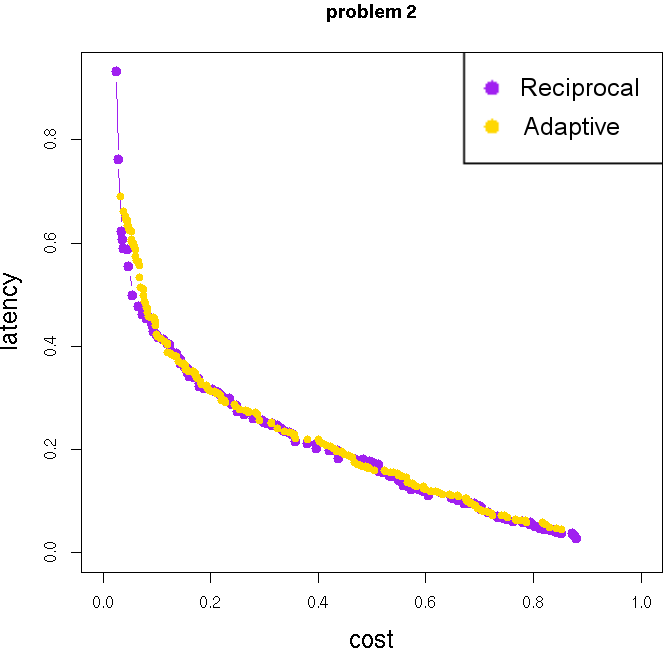
\includegraphics[width=\textwidth]{pics/transfer_problem2.png}
	   \caption{}
   \end{subfigure}
   \begin{subfigure}{0.49\textwidth}
       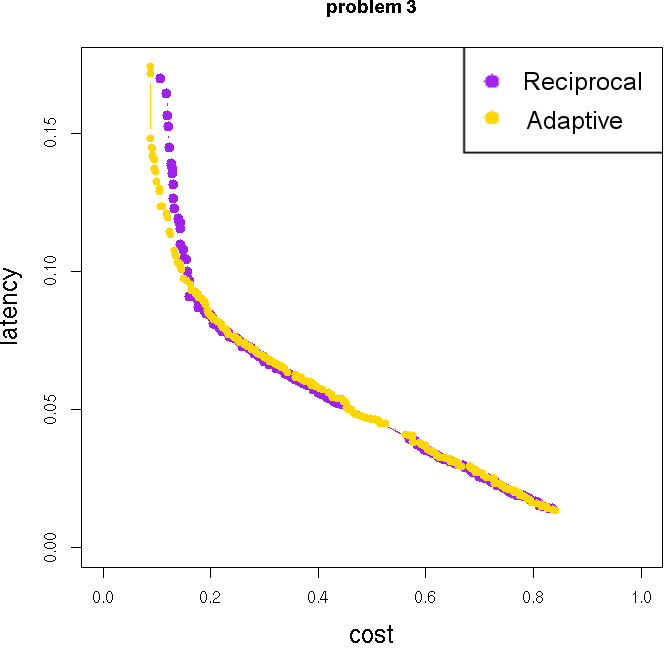
\includegraphics[width=\textwidth]{pics/transfer_problem3.png}
	   \caption{}
   \end{subfigure}
   \begin{subfigure}{0.49\textwidth}
       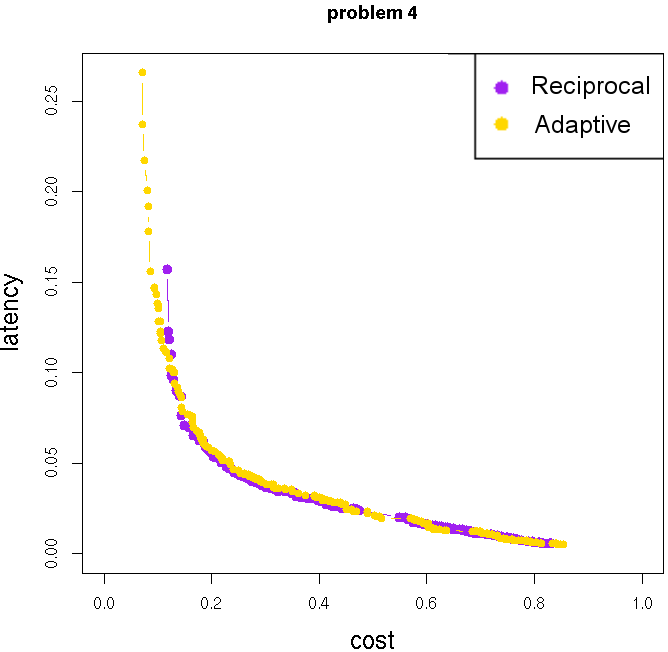
\includegraphics[width=\textwidth]{pics/transfer_problem4.png}
	   \caption{}
   \end{subfigure}
   \begin{subfigure}{0.49\textwidth}
       \includegraphics[width=\textwidth]{pics/transfer_problem5.png}
	   \caption{}
   \end{subfigure}
   \caption{Adaptive Rounding Function Experiments: The non-dominated solutions among the sets obtained by 40 independent runs of adaptive function and reciprocal
   function}
   \label{fig:transfer}
\end{figure}

\subsubsection{A Combination of Static Function}
In this experiment, we combined all solutions from 5 static rounding functions mentioned in Section \ref{sec:static_exp} and applied
a fast non-dominated sorting over it. The performance is compared with reciprocal rounding function in Figure \ref{fig:combination}.
As the figure shows, the combined non-dominated set dominates all problems. The solution is not only diverse but also uniformly distributed.
However, the major problem is that this method takes five times longer execution time than using reciprocal function.

\begin{figure}[h!]
   \centering
   \begin{subfigure}{0.49\textwidth}
       \includegraphics[width=\textwidth]{pics/combination_problem2.png}
	   \caption{}
   \end{subfigure}
   \begin{subfigure}{0.49\textwidth}
       \includegraphics[width=\textwidth]{pics/combination_problem3.png}
	   \caption{}
   \end{subfigure}
   \begin{subfigure}{0.49\textwidth}
       \includegraphics[width=\textwidth]{pics/combination_problem4.png}
	   \caption{}
   \end{subfigure}
   \begin{subfigure}{0.49\textwidth}
       \includegraphics[width=\textwidth]{pics/combination_problem5.png}
	   \caption{}
   \end{subfigure}
   \caption{Combination of Static Function Experiments:  The non-dominated solutions among
the sets obtained by 40 independent runs of combination of static thresholds and reciprocal
function}
   \label{fig:combination}
\end{figure}



\subsection{BMOPSOCD versus NSPSO, NSGA-II and BPSO}
The result is shown in Table \ref{tab:results}. In this table, ``Ave-'', ``Std-'' illustrate the average and standard deviation 
of four approaches over the 40 independent runs.
It can be seen from Table \ref{tab:results}, on all datasets except one, BMOPSOCD dominates other algorithms in both hypervolume and IGD. The only exception
is Problem 1, where BPSO has the best hypervolume value. On all datasets, only BMOPSOCD remains a good performance on hypervolume where there are obvious decreasing
trends in other three algorithms along with the number of variable increases. On all datasets, BMOPSOCD achieved a considerably better performance than other three
algorithms in IGD which indicates a high coverage.

In comparison with NSPSO and NSGA-II, BMOPSOCD with dynamic rounding function achieved significantly better convergence and diversity. The first reason is that with the dynamic
rounding function, BMOPSOCD could move out of local optima. In contrast, NSGA-II and NSPSO are easy to stuck at local optima. The second reason is BMOPSOCD 
keeps an external archive. Although three algorithms maintain a same size population, they produce different sizes of solutions. 
MOSPCOD outputs an archive with a size of 250 while other two algorithms output a population of size 50.

In Problem 1, the convergence of BMOPSOCD is worse than BPSO. One reason is probably that BPSO runs 50 generations with the same weight for both objectives,
it has more time to search a direction. On the other hand, with dynamic rounding function, MOSPCOD might not completely converge. Another reason is related to 
the variable size, where BPSO has better performance in small datasets, when the number of datasets increases, the performance drops rapidly. In contrast, 
BMOPSOCD with the dynamic rounding function is not affected by the variable sizes.
\begin{table}[!htb]
\centering
\footnotesize
\caption{Comparison between BMOPSOCD, NSPSO, NSGA-II and BPSO: The non-dominated solutions among the sets obtained by 40 independent runs of different algorithms}
\label{tab:results}

\begin{tabular}{|c|l|c|c|}
\hline
Dataset                         & \multicolumn{1}{c|}{Method}                                              & Hypervolume (avg $\pm$ sd)                                                                                                     & \multicolumn{1}{l|}{IGD (avg $\pm$ sd)}                                                                                                    \\ \hline
problem 1                       & \begin{tabular}[c]{@{}l@{}}BMOPSOCD\\ NSPSO\\ NSGA-II\\ BPSO\end{tabular} & \begin{tabular}[c]{@{}c@{}}0.83 $\pm$ 0.04\\ 0.76 $\pm$ 0.018\\ 0.83 $\pm$ 0.013\\ \textbf{0.89 $\pm$ 0.015} \end{tabular}  & \begin{tabular}[c]{@{}c@{}}\textbf{3.73E-02 $\pm$ 1.03E-02} \\ 0.16 $\pm$ 3.45E-02\\  0.19 $\pm$ 3.21E-02\\ 0.46 $\pm$ 2.45E-02\end{tabular} \\ \hline
problem 2                       & \begin{tabular}[c]{@{}l@{}}BMOPSOCD\\ NSPSO\\ NSGA-II\\ BPSO\end{tabular} & \begin{tabular}[c]{@{}c@{}}\textbf{0.73 $\pm$ 0.011} \\ 0.61 $\pm$ 0.001\\ 0.60 $\pm$ 0.011\\  0.61 $\pm$ 0.001\end{tabular} & \begin{tabular}[c]{@{}c@{}}\textbf{3.15E-02 $\pm$ 7.92E-03} \\ 0.15 $\pm$ 1.46E-02\\ 0.19 $\pm$ 1.81E-02\\  0.42 $\pm$ 1.54E-02\end{tabular} \\ \hline
problem 3                       & \begin{tabular}[c]{@{}l@{}}BMOPSOCD\\ NSPSO\\ NSGA-II\\ BPSO\end{tabular} & \begin{tabular}[c]{@{}c@{}}\textbf{0.81 $\pm$ 0.012} \\ 0.61 $\pm$ 0.011\\ 0.59 $\pm$ 0.008\\ 0.69 $\pm$ 0.007\end{tabular}  & \begin{tabular}[c]{@{}c@{}}\textbf{7.03E-03 $\pm$ 1.92E-03} \\ 0.10 $\pm$ 6.35E-03\\ 0.16 $\pm$ 7.25E-03\\  0.30 $\pm$ 8.94E-03\end{tabular} \\ \hline
problem 4                       & \begin{tabular}[c]{@{}l@{}}BMOPSOCD\\ NSPSO\\ NSGA-II\\ BPSO\end{tabular} & \begin{tabular}[c]{@{}c@{}}\textbf{0.83 $\pm$ 0.016} \\ 0.63 $\pm$ 0.012\\ 0.61 $\pm$ 0.008\\ 0.71 $\pm$ 0.008\end{tabular}  & \begin{tabular}[c]{@{}c@{}}\textbf{5.80E-03 $\pm$ 1.37E-03} \\ 0.11 $\pm$ 8.55E-03\\ 0.17 $\pm$ 9.11E-03 \\ 0.30 $\pm$ 8.62E-03\end{tabular} \\ \hline
problem 5                       & \begin{tabular}[c]{@{}l@{}}BMOPSOCD\\ NSPSO\\ NSGA-II\\ BPSO\end{tabular} & \begin{tabular}[c]{@{}c@{}}\textbf{0.84 $\pm$ 0.014} \\ 0.61 $\pm$ 0.009\\ 0.58 $\pm$ 0.005\\ 0.67 $\pm$ 0.007\end{tabular}  & \begin{tabular}[c]{@{}c@{}}\textbf{3.74E-03 $\pm$ 1.02E-03} \\ 0.11 $\pm$ 7.93E-03\\ 0.17 $\pm$ 6.89E-03\\  0.24 $\pm$ 5.02E-03\end{tabular} \\ \hline
\multicolumn{1}{|l|}{problem 6} & \begin{tabular}[c]{@{}l@{}}BMOPSOCD\\ NSPSO\\ NSGA-II\\ BPSO\end{tabular} & \begin{tabular}[c]{@{}c@{}}\textbf{0.81 $\pm$ 0.014} \\ 0.59 $\pm$ 0.007\\ 0.55 $\pm$ 0.006\\ 0.63 $\pm$ 0.005\end{tabular}  & \begin{tabular}[c]{@{}c@{}}\textbf{5.81E-03 $\pm$ 1.95E-03} \\ 0.11 $\pm$ 5.06E-03\\ 0.18 $\pm$ 8.01E-03 \\ 0.28 $\pm$ 5.88E-03\end{tabular} \\ \hline
problem 7                       & \begin{tabular}[c]{@{}l@{}}BMOPSOCD\\ NSPSO\\ NSGA-II\\ BPSO\end{tabular} & \begin{tabular}[c]{@{}c@{}}\textbf{0.79 $\pm$ 0.015} \\ 0.60 $\pm$ 0.008\\ 0.56 $\pm$ 0.005\\ 0.63 $\pm$ 0.006\end{tabular}  & \begin{tabular}[c]{@{}c@{}}\textbf{7.13E-03 $\pm$ 1.70E-03} \\ 0.10 $\pm$ 4.58E-03\\ 0.17 $\pm$ 6.48E-03 \\ 0.27 $\pm$ 7.92E-03\end{tabular} \\ \hline
problem 8                       & \begin{tabular}[c]{@{}l@{}}BMOPSOCD\\ NSPSO\\ NSGA-II\\ BPSO\end{tabular} & \begin{tabular}[c]{@{}c@{}}\textbf{0.81 $\pm$ 0.015} \\ 0.61 $\pm$ 0.008\\ 0.58 $\pm$ 0.005\\ 0.65 $\pm$ 0.007\end{tabular}  & \begin{tabular}[c]{@{}c@{}}\textbf{8.77E-03 $\pm$ 1.90E-03} \\ 0.12 $\pm$ 5.81E-03\\ 0.19 $\pm$ 6.17E-03 \\ 0.27 $\pm$ 5.86E-03\end{tabular} \\ \hline
problem 9                       & \begin{tabular}[c]{@{}l@{}}BMOPSOCD\\ NSPSO\\ NSGA-II\\ BPSO\end{tabular} & \begin{tabular}[c]{@{}c@{}}\textbf{0.83 $\pm$ 0.016} \\ 0.60 $\pm$ 0.009\\ 0.56 $\pm$ 0.004\\ 0.62 $\pm$ 0.005\end{tabular}  & \begin{tabular}[c]{@{}c@{}}\textbf{3.58E-03 $\pm$ 1.53E-03} \\ 0.11 $\pm$ 5.33E-03\\ 0.17 $\pm$ 3.56E-03 \\ 0.22 $\pm$ 3.22E-03\end{tabular} \\ \hline
problem 10                      & \begin{tabular}[c]{@{}l@{}}BMOPSOCD\\ NSPSO\\ NSGA-II\\ BPSO\end{tabular} & \begin{tabular}[c]{@{}c@{}}\textbf{0.80 $\pm$ 0.012} \\ 0.58 $\pm$ 0.008\\ 0.53 $\pm$ 0.005\\ 0.58 $\pm$ 0.005\end{tabular}  & \begin{tabular}[c]{@{}c@{}}\textbf{4.30E-03 $\pm$ 1.75E-03} \\ 0.11 $\pm$ 4.97E-03\\ 0.19 $\pm$ 5.62E-03 \\ 0.25 $\pm$ 3.91E-03\end{tabular} \\ \hline
problem 11                      & \begin{tabular}[c]{@{}l@{}}BMOPSOCD\\ NSPSO\\ NSGA-II\\ BPSO\end{tabular} & \begin{tabular}[c]{@{}c@{}}\textbf{0.79 $\pm$ 0.012} \\ 0.57 $\pm$ 0.009\\ 0.52 $\pm$ 0.003\\ 0.55 $\pm$ 0.003\end{tabular} & \begin{tabular}[c]{@{}c@{}}\textbf{5.19E-03 $\pm$ 1.81E-03} \\ 0.12 $\pm$ 4.22E-03\\ 0.20 $\pm$ 2.74E-03 \\ 0.24 $\pm$ 3.36E-03\end{tabular} \\ \hline
problem 12                      & \begin{tabular}[c]{@{}l@{}}BMOPSOCD\\ NSPSO\\ NSGA-II\\ BPSO\end{tabular} & \begin{tabular}[c]{@{}c@{}}\textbf{0.80 $\pm$ 0.01} \\ 0.58 $\pm$ 0.009\\ 0.52 $\pm$ 0.003\\ 0.56 $\pm$ 0.003\end{tabular} & \begin{tabular}[c]{@{}c@{}}\textbf{3.12E-03 $\pm$ 6.71E-04} \\ 0.12 $\pm$ 4.15E-03\\ 0.20 $\pm$ 3.08E-03 \\ 0.24 $\pm$ 2.50E-03\end{tabular} \\ \hline
problem 13                      & \begin{tabular}[c]{@{}l@{}}BMOPSOCD\\ NSPSO\\ NSGA-II\\ BPSO\end{tabular} & \begin{tabular}[c]{@{}c@{}}\textbf{0.83 $\pm$ 0.012} \\ 0.59 $\pm$ 0.008\\ 0.53 $\pm$ 0.003\\ 0.56 $\pm$ 0.004\end{tabular} & \begin{tabular}[c]{@{}c@{}}\textbf{2.63E-03 $\pm$ 6.73E-04} \\ 0.12 $\pm$ 3.46E-03\\ 0.20 $\pm$ 3.04E-03 \\ 0.22 $\pm$ 2.01E-03\end{tabular} \\ \hline
problem 14                      & \begin{tabular}[c]{@{}l@{}}BMOPSOCD\\ NSPSO\\ NSGA-II\\ BPSO\end{tabular} & \begin{tabular}[c]{@{}c@{}}\textbf{0.84 $\pm$ 0.015} \\ 0.59 $\pm$ 0.009\\ 0.53 $\pm$ 0.002\\ 0.57 $\pm$ 0.003\end{tabular} & \begin{tabular}[c]{@{}c@{}}\textbf{3.66E-03 $\pm$ 1.75E-03} \\ 0.13 $\pm$ 3.85E-03\\ 0.22 $\pm$ 3.24E-03 \\ 0.25 $\pm$ 1.83E-03\end{tabular} \\ \hline
\end{tabular}

\end{table}

In terms of execution time, although BMOPSOCD is not as good as NSGA-II, it achieves best or the second best for 11 out of 14 
problems (Table \ref{tab:time}).


\begin{table}[]
\centering
\footnotesize
\caption{Execution time}
\label{tab:time}
\scalebox{0.9}{

\begin{subtable}{.43\linewidth}
\centering
\begin{tabular}{|l|c|c|}
\hline
           & method                                                                   & time (avg $\pm$ sd)                                                                                                                           \\ \hline
problem 1  & \begin{tabular}[c]{@{}c@{}}BPSO\\ BMOPSOCD\\ NSPSO\\ NSGA-II\end{tabular} & \begin{tabular}[c]{@{}c@{}}17.99 $\pm$ 0.26 \\ \textbf{12.98 $\pm$ 0.18}\\ 19.00 $\pm$ 0.17 \\ 15.35 $\pm$ 0.15\end{tabular}                    \\ \hline
problem 2  & \begin{tabular}[c]{@{}c@{}}BPSO\\ BMOPSOCD\\ NSPSO\\ NSGA-II\end{tabular} & \begin{tabular}[c]{@{}c@{}}23.55 $\pm$ 0.27 \\ \textbf{16.18 $\pm$ 0.26}\\ 25.52 $\pm$ 0.27 \\ 15.38 $\pm$ 0.31\end{tabular}                    \\ \hline
problem 3  & \begin{tabular}[c]{@{}c@{}}BPSO\\ BMOPSOCD\\ NSPSO\\ NSGA-II\end{tabular} & \begin{tabular}[c]{@{}c@{}}103.65 $\pm$ 1.87 \\ 94.98 $\pm$ 7.28 \\ 111.86 $\pm$ 1.11 \\ \textbf{74.34 $\pm$ 0.61}\end{tabular}                 \\ \hline
problem 4  & \begin{tabular}[c]{@{}c@{}}BPSO\\ BMOPSOCD\\ NSPSO\\ NSGA-II\end{tabular} & \begin{tabular}[c]{@{}c@{}}181.20 $\pm$ 4.40 \\ 175.99 $\pm$ 9.67 \\ 182.09 $\pm$ 1.86 \\ \textbf{147.98 $\pm$ 1.30}\end{tabular}               \\ \hline
problem 5  & \begin{tabular}[c]{@{}c@{}}BPSO\\ MOPSOCD\\ NSPSO\\ NSGA-II\end{tabular} & \begin{tabular}[c]{@{}c@{}}137.03 $\pm$ 0.87 \\ 89.74 $\pm$ 8.53 \\ 161.31 $\pm$ 0.95 \\ \textbf{84.17 $\pm$ 1.03}\end{tabular}                 \\ \hline
problem 6  & \begin{tabular}[c]{@{}c@{}}BPSO\\ BMOPSOCD\\ NSPSO\\ NSGA-II\end{tabular} & \begin{tabular}[c]{@{}c@{}}208.63 $\pm$ 2.23 \\ 172.80 $\pm$ 7.68 \\ 236.23 $\pm$ 2.72 \\ \textbf{157.52$\pm$ 1.62}\end{tabular}                \\ \hline
problem 7  & \begin{tabular}[c]{@{}c@{}}BPSO\\ BMOPSOCD\\ NSPSO\\ NSGA-II\end{tabular} & \begin{tabular}[c]{@{}c@{}}234.73 $\pm$ 6.42 \\ 202.68 $\pm$ 10.46 \\ 242.94 $\pm$ 9.00 \\ \textbf{159.26 $\pm$ 1.31}\end{tabular}              \\ \hline
\end{tabular}
\end{subtable}

\begin{subtable}{.43\linewidth}
\centering
\begin{tabular}{|l|c|c|}
\hline
           & method                                                                   & time (avg $\pm$ sd)                                                                                                                           \\ \hline
problem 8  & \begin{tabular}[c]{@{}c@{}}BPSO\\ BMOPSOCD\\ NSPSO\\ NSGA-II\end{tabular} & \begin{tabular}[c]{@{}c@{}}476.76 $\pm$ 22.40 \\ 531.64 $\pm$ 43.14 \\ 444.41 $\pm$ 22.86 \\ \textbf{375.05 $\pm$ 4.11}\end{tabular}            \\ \hline
problem 9  & \begin{tabular}[c]{@{}c@{}}BPSO\\ BMOPSOCD\\ NSPSO\\ NSGA-II\end{tabular} & \begin{tabular}[c]{@{}c@{}}293.43 $\pm$ 3.01 \\ 198.81 $\pm$ 7.11 \\ 334.62 $\pm$ 2.81 \\ \textbf{181.30 $\pm$ 1.99}\end{tabular}               \\ \hline
problem 10 & \begin{tabular}[c]{@{}c@{}}BPSO\\ BMOPSOCD\\ NSPSO\\ NSGA-II\end{tabular} & \begin{tabular}[c]{@{}c@{}}507.72 $\pm$ 4.19 \\ 449.91 $\pm$ 26.00 \\ 539.51 $\pm$ 4.06 \\ \textbf{381.18 $\pm$ 3.06}\end{tabular}              \\ \hline
problem 11 & \begin{tabular}[c]{@{}c@{}}BPSO\\ BMOPSOCD\\ NSPSO\\ NSGA-II\end{tabular} & \begin{tabular}[c]{@{}c@{}}1,237.30 $\pm$ 42.06 \\ 1,262.79 $\pm$ 91.65\\ 1,328.17 $\pm$ 12.67 \\ \textbf{1,036.53 $\pm$ 35.38}\end{tabular}    \\ \hline
problem 12 & \begin{tabular}[c]{@{}c@{}}BPSO\\ BMOPSOCD\\ NSPSO\\ NSGA-II\end{tabular} & \begin{tabular}[c]{@{}c@{}}3,631.14 $\pm$ 17.70 \\ 4,326.22 $\pm$ 478.14 \\ 3,395.47 $\pm$ 100.51 \\ \textbf{3,326.94 $\pm$ 38.21}\end{tabular} \\ \hline
problem 13 & \begin{tabular}[c]{@{}c@{}}BPSO\\ BMOPSOCD\\ NSPSO\\ NSGA-II\end{tabular} & \begin{tabular}[c]{@{}c@{}}1,416.63 $\pm$ 0.26 \\ 1,155.21 $\pm$ 28.85 \\ 1,507.92 $\pm$ 25.74 \\ \textbf{1,098.08 $\pm$ 17.36}\end{tabular}    \\ \hline
problem 14 & \begin{tabular}[c]{@{}c@{}}BPSO\\ BMOPSOCD\\ NSPSO\\ NSGA-II\end{tabular} & \begin{tabular}[c]{@{}c@{}}3,617.53 $\pm$ 34.13 \\ \textbf{3,284.66 $\pm$ 124.13} \\ 3,759.51$\pm$ 61.49 \\ 3,372.53 $\pm$ 31.05 \end{tabular}   \\ \hline
\end{tabular}
\end{subtable}
}
\end{table}


\begin{figure}[]
   \caption{MOPSOCD, NSPSO and BPSO Experiments: The non-dominated solutions
among the sets obtained by 40 independent runs of different algorithms}
   \centering
   \begin{subfigure}{0.30\textwidth}
       \includegraphics[width=\textwidth]{pics/total1.png}
	   \caption{Problem 1}
   \end{subfigure}
   \begin{subfigure}{0.30\textwidth}
       \includegraphics[width=\textwidth]{pics/total2.png}
	   \caption{Problem 2}
   \end{subfigure}
   \begin{subfigure}{0.30\textwidth}
       \includegraphics[width=\textwidth]{pics/total3.png}
	   \caption{Problem 3}
   \end{subfigure}
      \begin{subfigure}{0.30\textwidth}
       \includegraphics[width=\textwidth]{pics/total4.png}
	   \caption{Problem 4}
   \end{subfigure}
      \begin{subfigure}{0.30\textwidth}
       \includegraphics[width=\textwidth]{pics/total5.png}
	   \caption{Problem 5}
   \end{subfigure}
   \begin{subfigure}{0.30\textwidth}
       \includegraphics[width=\textwidth]{pics/total6.png}
	   \caption{Problem 6}
   \end{subfigure}
   \begin{subfigure}{0.30\textwidth}
       \includegraphics[width=\textwidth]{pics/total7.png}
	   \caption{Problem 7}
   \end{subfigure}
      \begin{subfigure}{0.30\textwidth}
       \includegraphics[width=\textwidth]{pics/total8.png}
	   \caption{Problem 8}
   \end{subfigure}
      \begin{subfigure}{0.30\textwidth}
       \includegraphics[width=\textwidth]{pics/total9.png}
	   \caption{Problem 9}
   \end{subfigure}
   \begin{subfigure}{0.30\textwidth}
       \includegraphics[width=\textwidth]{pics/total10.png}
	   \caption{Problem 10}
   \end{subfigure}
   \begin{subfigure}{0.30\textwidth}
       \includegraphics[width=\textwidth]{pics/total11.png}
	   \caption{Problem 11}
   \end{subfigure}
   \begin{subfigure}{0.30\textwidth}
       \includegraphics[width=\textwidth]{pics/total12.png}
	   \caption{Problem 12}
   \end{subfigure}
      \begin{subfigure}{0.30\textwidth}
       \includegraphics[width=\textwidth]{pics/total13.png}
	   \caption{Problem 13}
   \end{subfigure}
      \begin{subfigure}{0.30\textwidth}
       \includegraphics[width=\textwidth]{pics/total14.png}
	   \caption{Problem 14}
   \end{subfigure}
   \label{fig:total}
\end{figure}

\subsection{Discussions}
In this chapter, we proposed a binary version of multi-objective PSO with crowding distance to solve the Web service location allocation problem.
The major contribution is that, we provide a rounding function and an adaptive threshold technique to make a continuous algorithm compatible with a binary problem.
These techniques can also be applied in other continuous algorithms.
BMOPSOCD shows 2 major desirable features. 
\begin{enumerate}
	\item The solution set has a good diversity which covers most of the Pareto front.
	\item BMOPSOCD could produce good solutions regardless of increasing problem size.
\end{enumerate}

\subsection{Summary}
This chapter proposed a BMOPSOCD to solve the Web service location allocation problem. We introduce a rounding function technique 
enables the continuous algorithm to handle binary problems. Meanwhile, an adaptive threshold embodies the idea of transfer
learning.
The proposed algorithm was compared with previous approaches. The results show that, on most datasets, BMOPSOCD can achieve much better results in both convergence and diversity than other three
methods, NSPSO, NSGA-II and BPSO. Additionally, the performance of MOSPCOD with dynamic rounding function is not affected by the size of variable. That is
a significantly improvement.


